\documentclass[11pt,a4paper]{article}
\usepackage{fontspec}
\setmainfont{Source Serif 4}[Path=/home/claude/ref/fonts/, UprightFont=SourceSerif4-Regular.ttf, BoldFont=SourceSerif4-Semibold.ttf, ItalicFont=SourceSerif4-It.ttf]
\setmonofont{IBM Plex Mono}[Path=/home/claude/ref/fonts/, UprightFont=IBMPlexMono-Regular.ttf, BoldFont=IBMPlexMono-Medium.ttf, Scale=0.88]
\usepackage[a4paper,margin=2.4cm]{geometry}
\usepackage{amsmath}
\usepackage{graphicx,booktabs,float,caption,array,xcolor,longtable}
\usepackage{xurl}
\usepackage[hidelinks]{hyperref}
\usepackage[round]{natbib}
\usepackage{setspace}
\setstretch{1.08}
\renewcommand{\topfraction}{0.9}
\renewcommand{\bottomfraction}{0.8}
\renewcommand{\textfraction}{0.1}
\renewcommand{\floatpagefraction}{0.75}
\setlength{\parindent}{0pt}
\setlength{\parskip}{0.55em}
\captionsetup{font=small,labelfont=bf}
\setlength{\bibsep}{3pt}
\urlstyle{same}
\hypersetup{pdftitle={Where Romans Wrote},pdfauthor={Dr Tristan Hotham}}

\begin{document}
\begin{center}
{\Large\bfseries Where Romans Wrote: The Epigraphic Habit, Age Rounding and Soldiers' Origins in 200,000 Latin Inscriptions\par}
\vspace{1.2em}
{\large Dr Tristan Hotham\par}
\vspace{0.3em}
{\small Independent researcher\\
ORCID: 0000-0003-4931-9349\\
DOI: https://doi.org/10.5281/zenodo.24114976\par}
\vspace{0.8em}
2026
\end{center}

\begin{quote}
\small
\begin{center}\textbf{Abstract}\end{center}
Latin inscriptions are the largest body of written evidence from the Roman Empire, and their aggregated databases now allow questions about the whole corpus to be asked with explicit statistical methods. I use LIRE, a harmonised dataset of 203,466 Latin inscriptions with findspots and date ranges, to test three long-standing claims, each pre-specified in a written plan before any outcome was computed. First, MacMullen's epigraphic habit: aoristic counts show that the number of inscriptions per year in AD 193 to 235 was 2.2 times that in 250 to 300 (Monte Carlo interval 2.16 to 2.24), but the empire-wide peak falls in AD 68, not under the Severans, because Rome and Italy, 61\% of the corpus, wrote most in the first century; 10 of 27 well-recorded provinces peak between 175 and 250. Second, age rounding on epitaphs: 29,598 stated ages give a Whipple index of 303 (95\% CI 298 to 307). Rounding rises with age and is heavier in the countryside than in large cities (odds ratio 1.50, 95\% CI 1.09 to 2.07), though not in every check; the expected excess in Africa over Rome is not significant once setting and age are held fixed (odds ratio 1.22, 0.88 to 1.68). Third, soldiers' stated origins on 865 military stones lie a median 674~km from the stone, and show no sign of the more local recruitment documented for the legions: stones from after AD 100 do not name nearer homes. Rules, validation samples and code are released.

\textbf{Keywords:} Latin epigraphy; epigraphic habit; aoristic analysis; age heaping; Whipple index; Roman army; recruitment; digital epigraphy
\end{quote}

\section{Introduction}
The Roman Empire left more inscribed text than any other ancient state, and most of it is Latin: epitaphs, dedications to gods, honours for patrons and emperors, building records, milestones and the small stamped and scratched texts of everyday objects. For a century and a half historians have used inscriptions one at a time, as documents. For about fifty years they have also counted them. \citet{mrozek1973} plotted the chronological distribution of dated Latin inscriptions; \citet{macmullen1982} named the ``epigraphic habit'', the rise of inscribing through the first and second centuries AD and its collapse after the Severan emperors; \citet{meyer1990} explained it through epitaphs and the value of Roman status; \citet{woolf1996} through monumental writing as a way of fixing one's place in a changing society. In demography, \citet{hopkins1966} showed why the ages on tombstones cannot be read as a life table, and \citet{duncanjones1977} read the rounding of those ages to multiples of five as evidence of how far people knew their exact age. In military history, the origins that soldiers gave on their tombstones were the basis of the classic studies of recruitment by \citet{forni1953} and \citet{mann1983}.

These studies were built on samples the authors assembled by hand, from the printed corpora, and they reported counts and percentages. The two large epigraphic databases, the Epigraphik-Datenbank Clauss/Slaby \citep[EDCS;][]{edcs} and the Epigraphic Database Heidelberg \citep[EDH;][]{edh}, now hold most published Latin inscriptions with findspots and editors' date ranges, and the LIRE dataset \citep{kase2023lire} merges and harmonises the two. It allows the same questions to be asked of the whole corpus at once, with methods that handle uncertain dates and clustered evidence, and with every rule written down. That is the contribution of this paper. It does not offer a new reading of any inscription. It asks whether three established claims hold when tested on 203,466 inscriptions with explicit, reproducible methods, and it reports where they do not.

The three tests are these. (1) Does the number of Latin inscriptions per year peak in the Severan period (AD 193 to 235) and fall sharply afterwards, as \citet{macmullen1982} argued? (2) Are the ages on epitaphs rounded everywhere, and is rounding heavier in Africa than in Rome, in the countryside than in large cities, and at higher ages, as \citet{duncanjones1977} suggested? (3) Do the origins stated by soldiers become more local over time, as the recruitment studies of \citet{forni1953} and \citet{mann1983} imply? Each hypothesis, its test and what would count against it were fixed in a written plan (released with the code) after inspecting only the structure of the data. The results are mixed, and the paper reports them as planned: the post-Severan collapse is very large, but the empire-wide peak is in the first century; rounding is universal and grows with age, but the African excess disappears once the setting of the stone is held fixed; and the soldiers' stated origins do not move closer to home.

Section~\ref{sec:lit} reviews the three literatures and the digital work on which this paper builds. Section~\ref{sec:data} describes the data and Section~\ref{sec:design} the methods and the plan. Section~\ref{sec:results} reports the results, Section~\ref{sec:robust} the checks, and Section~\ref{sec:disc} discusses what the evidence can and cannot show. Section~\ref{sec:conc} concludes.

\section{Background and literature}\label{sec:lit}
\subsection{The epigraphic habit}
\citet{macmullen1982} observed that the number of Latin inscriptions, counted by date, rises from Augustus to a peak in the early third century and falls steeply in the decades after AD 235, and that the fall is too general to be explained by the destruction of stones or the fortunes of single provinces. He suggested that inscribing depended on a ``sense of audience'' that faded in the third century. \citet{mrozek1973} had already shown a similar curve for dated inscriptions of the high empire. \citet{meyer1990}, working from epitaphs, linked the habit to the value of Roman legal status: commemoration in the Roman manner flourished where people held, or hoped to acquire, Roman status, and its decline followed the universal grant of citizenship in AD 212, which removed the distinction. \citet{woolf1996} widened the frame, reading monumental writing as a means by which individuals in a fast-changing imperial society fixed their identity and place in the world, so that its spread tracked the expansion of Roman society itself. \citet{beltran2014} surveys the debate and the regional variety of the habit, and the handbook in which his chapter appears \citep{bruun2014} gives the wider context of Latin epigraphy, including the army \citep{speidel2014}, mobility \citep{kolb2014}, literacy \citep{bodel2014} and the rise of Christian epigraphy \citep{mazzoleni2014}.

A curve of this kind depends on how inscriptions are dated. Most are not dated by an explicit year but by editors' ranges based on letter forms, formulae, names and archaeological context, and many ranges are long or conventional. The archaeological literature on temporal uncertainty offers two standard tools. Aoristic analysis spreads each item evenly over its date range \citep{ratcliffe2000,johnson2004}; Monte Carlo simulation draws a date within each range many times and so gives intervals for any statistic of the summed distribution \citep{crema2012}. \citet{baxtercool2016} discuss the same problem for brooches in Roman Britain and \citet{palmisano2017} compare such proxies for long-term population change in central Italy. The SDAM project, which produced LIRE, has used these tools on Latin inscriptions \citep{hermankova2021,kase2022division}.

\subsection{Ages on tombstones and age rounding}
Epitaphs often record the age of the dead, and early scholarship used them to estimate Roman life expectancy. \citet{hopkins1966} showed why this fails: the commemorated are not a random sample of the dead. Infants and young children are under-represented, men more often commemorated than women, and the age distributions implied by epitaphs vary between regions far more than any plausible mortality difference. \citet{scheidel2001} describes demographic analysis of epitaphs as now largely discredited, and the field turned to model life tables \citep{frier1982,frier1983,parkin1992,scheidel1996}. Epitaphs remain informative about commemoration itself: \citet{sallershaw1984} used who commemorated whom to study family relations among civilians, soldiers and slaves.

The rounding of ages is a separate question, and one the epitaphs can answer. \citet{duncanjones1977} showed that ages ending in 0 and 5 are far over-represented and argued that the degree of rounding measures how far people knew their exact age, with heavier rounding in Africa than in Rome, among lower social groups and at higher ages. The same idea underlies the use of age heaping as a measure of numeracy in economic history: \citet{ahearn2009} compile heaping indices for many populations, show that they correlate with literacy, and propose the ABCC index, a linear transformation of Whipple's index. \citet{myers1940} gives the blended index that uses all terminal digits. On Latin epitaphs the rounding may come from the deceased, the family or the stonecutter, and Roman numerals make multiples of five visually simple (V, X, L), so the index measures a habit of the commemorators as much as anyone's knowledge.

\subsection{Soldiers' origins and recruitment}
Roman soldiers' tombstones and dedications often state the man's origin: his home town (\textit{domo} followed by the town), his voting tribe and town, or his people (\textit{natione} followed by an ethnic adjective). \citet{forni1953} assembled such origins for legionaries and showed that recruitment shifted from Italy to the provinces in the first century AD and became increasingly local in the second and third centuries, with legions drawing on the provinces where they were stationed. \citet{mann1983} extended the analysis and linked it to veteran settlement. \citet{haynes2013} studies the auxilia, whose recruitment was also increasingly local after the early first century. In the city of Rome, origins on inscriptions are a main source for migration: \citet{noy2000} collects foreigners at Rome, and \citet{tacoma2016} models migration to the capital, where the praetorian guard, the imperial horse guard and the fleets at Misenum and Ravenna drew men from distant provinces.

\subsection{Digital epigraphy at scale}
\citet{hermankova2021} set out the case for treating inscriptions as data at a macro-historical scale and describe the processing of EDH and EDCS behind the SDAM datasets. \citet{kase2021classifying} trained a classifier that assigns EDH's inscription types to the EDCS-only records, which is how LIRE gives one typology to the whole corpus. \citet{kase2022division} used the same data to study occupations in Roman cities, using the city list of \citet{hanson2016} to set urban context, as LIRE does. The present paper uses that infrastructure for three classic questions, adds explicit extraction rules for ages and origins, and tests pre-specified hypotheses with methods that respect clustering and date uncertainty.

\subsection{What is new here}
To my knowledge no published study has (i) estimated the empire-wide and province-level timing of the Latin epigraphic habit on the full EDCS and EDH corpus with aoristic and Monte Carlo methods, (ii) tested the regional and social pattern of age rounding with a clustered model on all extractable ages, or (iii) mapped every military stone with a stated and identifiable origin. Each analysis follows a written plan fixed in advance, and each rule is released with code and validation samples.

\section{Data}\label{sec:data}
\subsection{LIRE}
LIRE v2.1 \citep{kase2023lire} contains 203,466 Latin inscriptions that have a findspot with coordinates and a date range overlapping 50 BC to AD 350. It merges EDCS (200,962 records) and EDH (64,869 records); inscriptions in both are merged into one row with the attributes of both. Each row has the edition text (in EDCS and EDH conventions, with expansions of abbreviations in round brackets and restorations in square brackets), a cleaned text, the province (EDCS province names, 65 values including the city of Rome and the eleven Augustan regions of Italy), the findspot name, an urban context (large, medium or small city, or rural, by distance to the cities of \citet{hanson2016}), the inscription type from EDH or from the classifier of \citet{kase2021classifying}, EDCS's category list (which marks, for example, epitaphs, soldiers and Christian inscriptions), and the date range \texttt{not\_before} to \texttt{not\_after}. 203,380 rows have both dates; the median range is 99 years. In 38 rows the two dates were in the wrong order and were swapped. LIRE is released under CC BY 4.0. The EDH \texttt{people} field gives names and sex, but no ages or origins, so ages and origins are read from the text (Section~\ref{sec:design}).

The corpus is very uneven (Table~\ref{tab:corpus}). The city of Rome has 75,301 inscriptions (37.0\%) and the rest of Italy 48,874; together 61.0\%. Of the 49,396 inscriptions in the EDCS category ``inscriptiones christianae'', 42,181 are from the city of Rome. Greek inscriptions are not in LIRE, so the eastern provinces, where Greek was the language of public writing, are represented only by their Latin minority.

\begin{table}[tbp]\centering\small\caption{The corpus by regional group (EDCS provinces grouped; Appendix B): inscriptions, share, inscriptions with a date range of 100 years or less (the main set of Part 1), epitaphs, extracted ages, and military stones with a mapped origin (by findspot).}\label{tab:corpus}\begin{tabular}{lrrrrrr}\toprule Group & Inscriptions & \% & Range $\leq$100 & Epitaphs & Ages & Soldiers\\\midrule
Rome & 75,301 & 37.0 & 54,721 & 61,938 & 10,583 & 310\\
Italy & 48,874 & 24.0 & 40,674 & 24,872 & 5,409 & 207\\
Africa & 8,219 & 4.0 & 6,685 & 5,287 & 4,086 & 20\\
Hispania & 11,467 & 5.6 & 9,100 & 6,097 & 2,578 & 3\\
Gaul and Germany & 16,329 & 8.0 & 10,648 & 5,002 & 857 & 102\\
Danube and Balkans & 29,387 & 14.4 & 16,484 & 13,411 & 5,256 & 179\\
Britain & 4,684 & 2.3 & 2,230 & 609 & 222 & 21\\
East & 2,948 & 1.4 & 2,705 & 289 & 92 & 16\\
Islands & 3,707 & 1.8 & 2,923 & 1,180 & 514 & 6\\
Other & 2,550 & 1.3 & 1,268 & 786 & 1 & 1\\
\midrule All & 203,466 & 100.0 & 147,438 & 119,471 & 29,598 & 865\\
\bottomrule\end{tabular}\end{table}

\subsection{Provinces and places}
For the map and for areas I use the Digital Atlas of the Roman Empire \citep[DARE;][]{ahlfeldt2013}: province polygons of about AD 117, with the Augustan regions of Italy, and a gazetteer of ancient places with Latin names and coordinates, as packaged in an open repository of DARE vector data. Each inscription is assigned to the DARE province containing its findspot (coastal points within about 25~km to the nearest), and the city of Rome is kept apart. The DARE provinces cover about 4,879,525~km$^2$. Province areas are approximate and the boundaries those of one date; densities are descriptive.

\section{Methods and analysis plan}\label{sec:design}
\subsection{Part 1: the epigraphic habit}
\textit{Aoristic counts.} Each dated inscription carries a weight of one, spread evenly over the years from \texttt{not\_before} to \texttt{not\_after} inclusive. Summing over inscriptions gives the expected number of inscriptions per year, from 50 BC to AD 400. The main set is the 147,438 inscriptions (72\% of the dated) whose range is 100 years or less; inscriptions with longer ranges add little information about timing and flatten the curve. The planned sensitivity sets are ranges of 50 years or less, 200 years or less, and all dated inscriptions.

\textit{Monte Carlo.} In each of 1,000 replicates every inscription is given one year drawn uniformly from its range; the replicate's peak year (of its 25-year moving mean) and its ratio below (on the unsmoothed annual counts, as for the point estimate) are recorded. The 2.5th and 97.5th percentiles give 95\% intervals.

\textit{H1a.} Following \citet{macmullen1982}, the 25-year moving mean of the main curve peaks in the Severan period, and the mean annual count in 193 to 235 is well above that in 250 to 300. The plan set the test: the peak year should fall in 175 to 250 and the ratio should be at least 1.5; a peak outside that window or a ratio under 1.5 counts against H1a.

\textit{H1b.} Descriptive: the peak year with Monte Carlo intervals for each type of inscription (by LIRE's type) and for each EDCS province with at least 1,000 inscriptions in the main set, and the curves of eight regional groups (Rome; the rest of Italy; Africa; Hispania; Gaul and the Germanies; the Danube and Balkan provinces; Britain; the Greek East).

\subsection{Part 2: ages at death}
\textit{Extraction.} The rule was fixed before any age was looked at. In the edition text, expansions are resolved (\texttt{ann(is)} becomes \textit{annis}), editorial corrections take the corrected reading, superfluous letters are dropped and line breaks are joined (so that a numeral split across lines is read whole). A stated age is a word of the form \textit{an, ann, annis, annos, annorum, anno, annum} followed by an intact Roman numeral, either after a form of \textit{vixit} in the two words before (form A) or in the genitive \textit{annorum} (``aged'', form B). The numeral must contain no restored letter or query; it is parsed as written on stone, including additive forms (IIII, VIIII, XXXX) and the subtractive forms IIX (8) and XXC (80). Two exclusions keep out years that are not ages: years of service (a word beginning \textit{milit-}, \textit{stip-}, \textit{aer-}, \textit{meru-}, \textit{emerit-} in the three words before) and years of marriage (\textit{cum qua vixit annis}, \textit{vixit mecum}). The phrase \textit{plus minus} between the word and the numeral is allowed and flagged. Ages from 0 to 110 are kept. Only epitaphs count (LIRE type epitaph or EDCS category ``tituli sepulcrales''). Several ages on one stone are kept; the stone is the unit of resampling.

Reading the first validation sample led to four fixes, made before any distribution was computed: the marriage exclusion, the strict numeral parser, accepting a restored letter in the word for years (not in the numeral) and reading ages after \textit{plus minus}. With the final rule, 200 randomly sampled extracted ages were read against the text: 199 were ages at death as written, and one counted years lived after a patron's death. Of 100 randomly sampled epitaphs with no extracted age, 5 state an age legibly: 2 that the rule should have read and 3 in forms outside it (ages in words, or without \textit{vixit}).

\textit{Measures.} Whipple's index on ages 23 to 62 is $W = 500 \times$ (share of ages ending in 0 or 5); $W = 100$ means no preference for those digits and $W = 500$ means every age is a multiple of five. The ABCC index of \citet{ahearn2009} is $100\,(1 - (W-100)/400)$. Confidence intervals come from 1,000 bootstrap resamples of stones. Myers' blended index \citep{myers1940} on ages 10 to 89 is reported as an alternative measure.

\textit{Hypotheses.} H2a: $W > 100$ in every regional group with at least 200 ages in the range (against: any interval including 100). H2b \citep{duncanjones1977}: rounding is heavier in Africa (Africa Proconsularis, Numidia and the two Mauretanias) than in the city of Rome. H2c: rounding is heavier in rural than in large urban contexts. H2d: rounding rises with age. The planned model is a logistic regression of whether an age (23 to 62) is a multiple of five on regional group (reference: Rome), urban context (reference: large), age band (23 to 32, 33 to 42, 43 to 52, 53 to 62) and whether the inscription is Christian, with standard errors clustered by findspot (the EDCS place name, or the point where none is given). H2b and H2c are supported if the lower bound of the 95\% interval of the relevant odds ratio is above 1; H2d if the odds ratios of the age bands rise. Planned robustness checks: ages 23 to 72; form A only; excluding Christian inscriptions; one age per stone; excluding \textit{plus minus} ages; leaving out each regional group in turn.

\textit{Life expectancy.} No estimate is made. Following \citet{hopkins1966}, I report the mean age, the share under ten and the number of ages of 100 or more by region, to show why the stones are not a life table.

\subsection{Part 3: soldiers' origins}
\textit{Military stones.} An inscription is military if EDCS lists it under ``milites'' or its text contains a military word (\textit{miles, legionis, cohortis, ala, eques, veteranus, centurio, signifer, beneficiarius, optio, praetorianus, classis, stipendiorum, militavit, evocatus} and similar). This includes officers and senators whose careers name a legion. Military diplomas are kept apart, because the origin they give is the recipient's home and they are often found there.

\textit{Origins.} Four forms are read from the text: \textit{domo} X (a tribe name before a town is skipped), \textit{natione} X, \textit{civis} X, and a voting tribe directly after the filiation (\textit{filius} or \textit{f.}) followed within three words by a town (\textit{Pollia Mutina}, ``of the tribe Pollia, from Mutina''). Restored or queried words are not read. Ethnic adjectives (\textit{Bessus}, \textit{Thrax}, \textit{Syrus}, \textit{Pannonius}, \textit{Batavus}...) are mapped by hand to a point for the people or region, flagged as regional (code/natio.csv). Town names are matched to the DARE gazetteer through their usual case forms (\textit{Mediolano} to \textit{Mediolanum}); automatic matches are allowed only against DARE settlements in or near the empire, a word that is also a common personal name in EDH is matched only to a major town, and a form that points to several places more than 50~km apart is ambiguous and dropped. Every origin form used at least twice (126 forms) was read in context and either confirmed, mapped by hand or rejected (code/origo\_overrides.csv); in a sample of 60 forms used once, 4 were wrong and were corrected. The outcome is the great-circle distance from the origin to the findspot.

\textit{H3} \citep{forni1953,mann1983}: soldiers' stated origins become more local over time. The planned test compares stones dated wholly before AD 101 (\texttt{not\_after} $\leq 100$) with stones dated wholly within AD 101 to 300, by median (quantile) regression of log distance on the later period, with a cluster bootstrap over findspots (1,000 replicates) for the interval. H3 is supported if the ratio of medians (later over earlier) has an upper bound below 1. Planned checks: town origins only; excluding findspots in Rome; excluding Rome and Italy; date ranges of 100 years or less. The plan also said that if fewer than 300 stones had a mapped origin, Part 3 would be descriptive only.

\section{Results}\label{sec:results}
\subsection{Where the inscriptions are}
Figure~\ref{fig:map} maps the corpus. Outside Rome and Italy, the densest areas are the Rhine frontier around Mainz, the coast of Dalmatia around Salona, the cities of Africa Proconsularis and Numidia, southern Spain, and the Danube frontier. Across the DARE provinces there are 26.1 inscriptions per 1,000~km$^2$ excluding the city of Rome; the Italian region around Rome and Campania (Regio~I) has 1,379, Britain 27.7, and the Latin record of the eastern provinces is thin (Galatia and Cappadocia 2.0). Of all inscriptions 40\% are in large urban contexts and 22\% rural.

\begin{figure}[tbp]\centering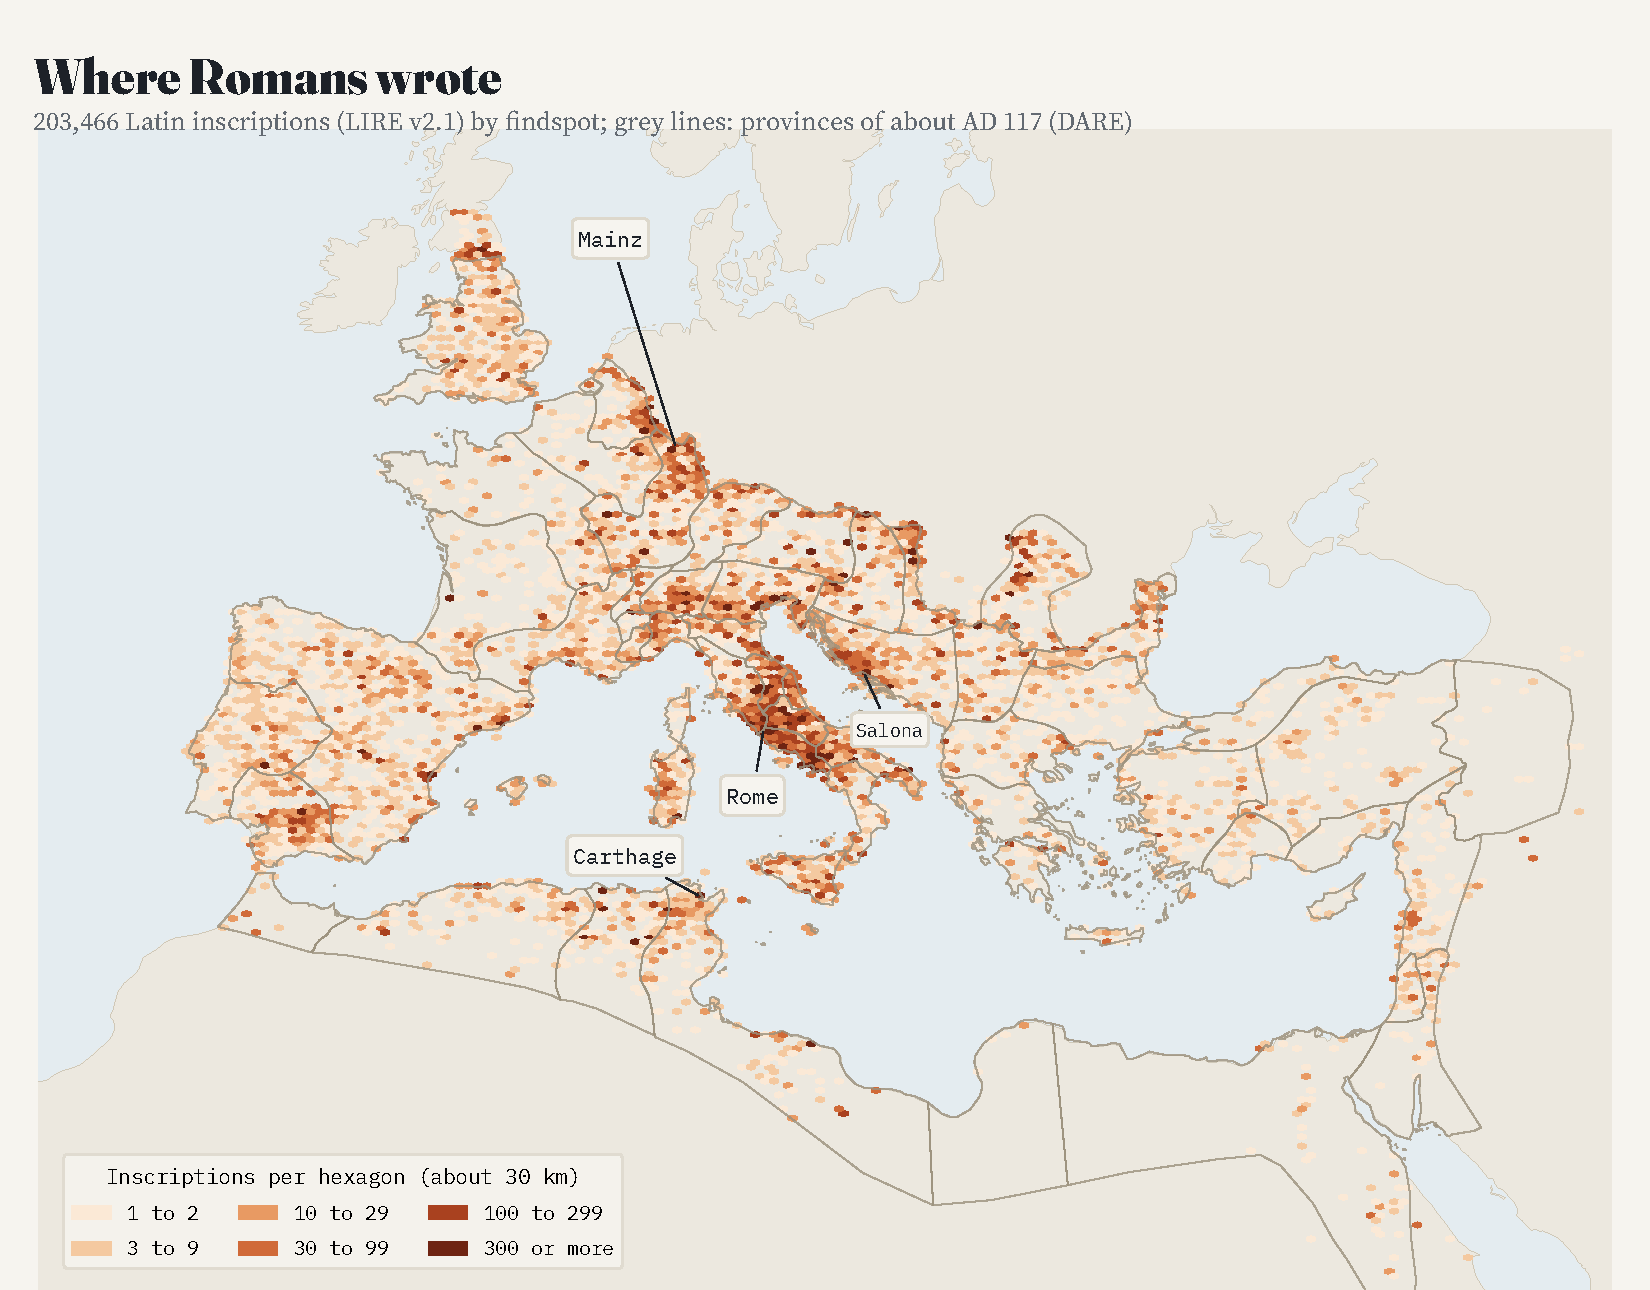
\includegraphics[width=\textwidth]{f_map.pdf}\caption{Latin inscriptions in LIRE v2.1 by findspot, in hexagons about 30~km across (Lambert azimuthal equal-area projection). Grey lines: DARE provinces of about AD 117.}\label{fig:map}\end{figure}

\subsection{H1: the epigraphic habit}
Figure~\ref{fig:time} shows the main curve. It rises from the late first century BC to a plateau in the first and second centuries AD and falls after about AD 230 to a trough in the later third century, before a fourth-century recovery driven by Christian epitaphs. The mean annual count in 193 to 235 is 353 and in 250 to 300 161: a ratio of 2.20 (Monte Carlo 95\% interval 2.16 to 2.24), a fall of 55\%. Excluding Christian inscriptions the ratio is 3.2. The collapse that MacMullen described is therefore very large and robust to every dating set (Table~\ref{tab:habit}).

The peak, however, is not Severan. The 25-year moving mean peaks in AD 68 (Monte Carlo 95\% interval AD 13 to 71), and in AD 128 when all dated inscriptions are used. By the planned rule H1a is therefore not supported empire-wide: the peak lies outside 175 to 250 even though the fall exceeds the planned threshold. The mean over the first century (425 per year) is higher than over the second (374) and the third (234). Two visible spikes are artefacts of exact dates: 4,166 inscriptions from the Vesuvian cities end in AD 79, and 1,304 items are dated to AD 123, 971 of them in Rome and 1,062 identification or owner inscriptions (stamped bricks and objects).

\begin{figure}[tbp]\centering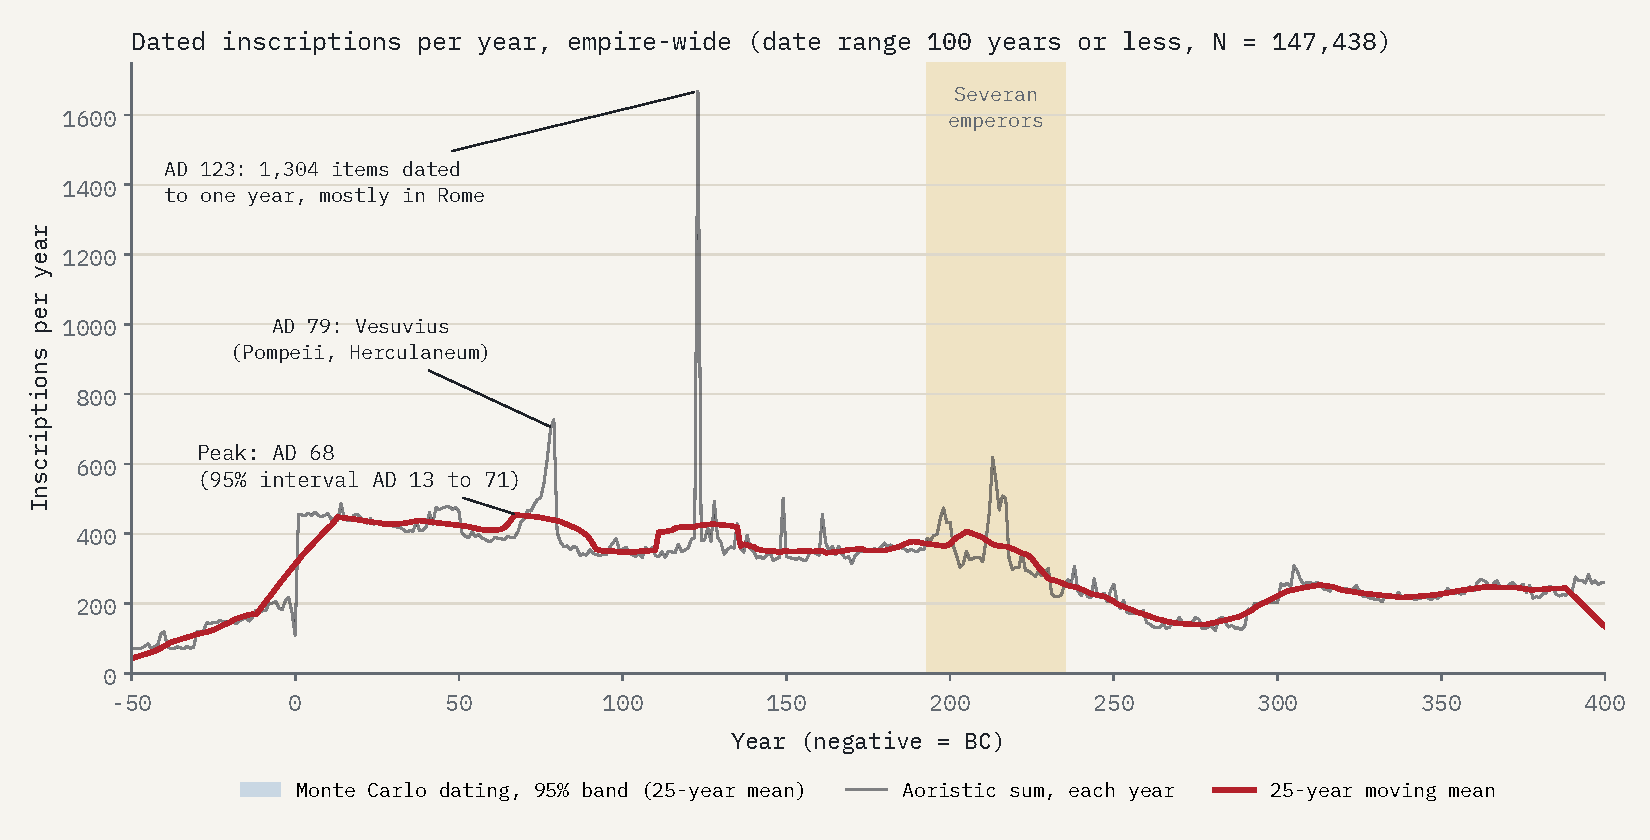
\includegraphics[width=\textwidth]{f_time.pdf}\caption{Dated Latin inscriptions per year (aoristic sum, range 100 years or less), with the 25-year moving mean and the Monte Carlo 95\% band of the smoothed curve. Shaded: the Severan emperors, AD 193 to 235.}\label{fig:time}\end{figure}

\begin{table}[tbp]\centering\small\caption{H1a. Peak year of the 25-year moving mean of the aoristic sum, and the ratio of the mean annual count in AD 193 to 235 to that in 250 to 300, by dating set. Brackets: Monte Carlo 95\% intervals. The planned test required a peak in 175 to 250 and a ratio of at least 1.5.}\label{tab:habit}\begin{tabular}{lrrr}\toprule Dating set & N & Peak (AD) & Ratio 193 to 235 / 250 to 300\\\midrule
Range 100 years or less (main) & 147,438 & 68 & 2.20\\
Range 50 years or less & 74,295 & 68 & 2.16\\
Range 200 years or less & 194,507 & 128 & 1.92\\
All dated & 203,380 & 128 & 1.83\\
Main set, Monte Carlo (1,000 draws) & 147,438 & 68 [13, 71] & 2.20 [2.16, 2.24]\\
\bottomrule\end{tabular}\end{table}

Why does the empire-wide peak fall so early? Figure~\ref{fig:groups} shows the curve of each regional group. Rome and the rest of Italy, 61\% of the corpus, peak in the first century AD and decline slowly through the second; their weight sets the empire-wide shape. The provinces differ. Africa and the Danube and Balkan provinces rise through the second century to a sharp Severan maximum and collapse after it; Gaul and the Germanies have a first-century peak (the early army on the Rhine) and a second, Severan one; Hispania peaks in the late first century; Britain in the second quarter of the second century. Province by province (Table~\ref{tab:peaks} and Figure~\ref{fig:peaks}), 10 of the 27 provinces with at least 1,000 inscriptions in the main set peak between 175 and 250: Africa Proconsularis, Numidia, Mauretania Caesariensis, Baetica, Dacia, Noricum, the two Pannonias, Germania inferior and Dalmatia (the last two with wide intervals). The Italian regions and Narbonensis peak between the late first century BC and the later first century AD, and the city of Rome in the late fourth century, when its Christian catacomb epitaphs are dated.

\begin{figure}[tbp]\centering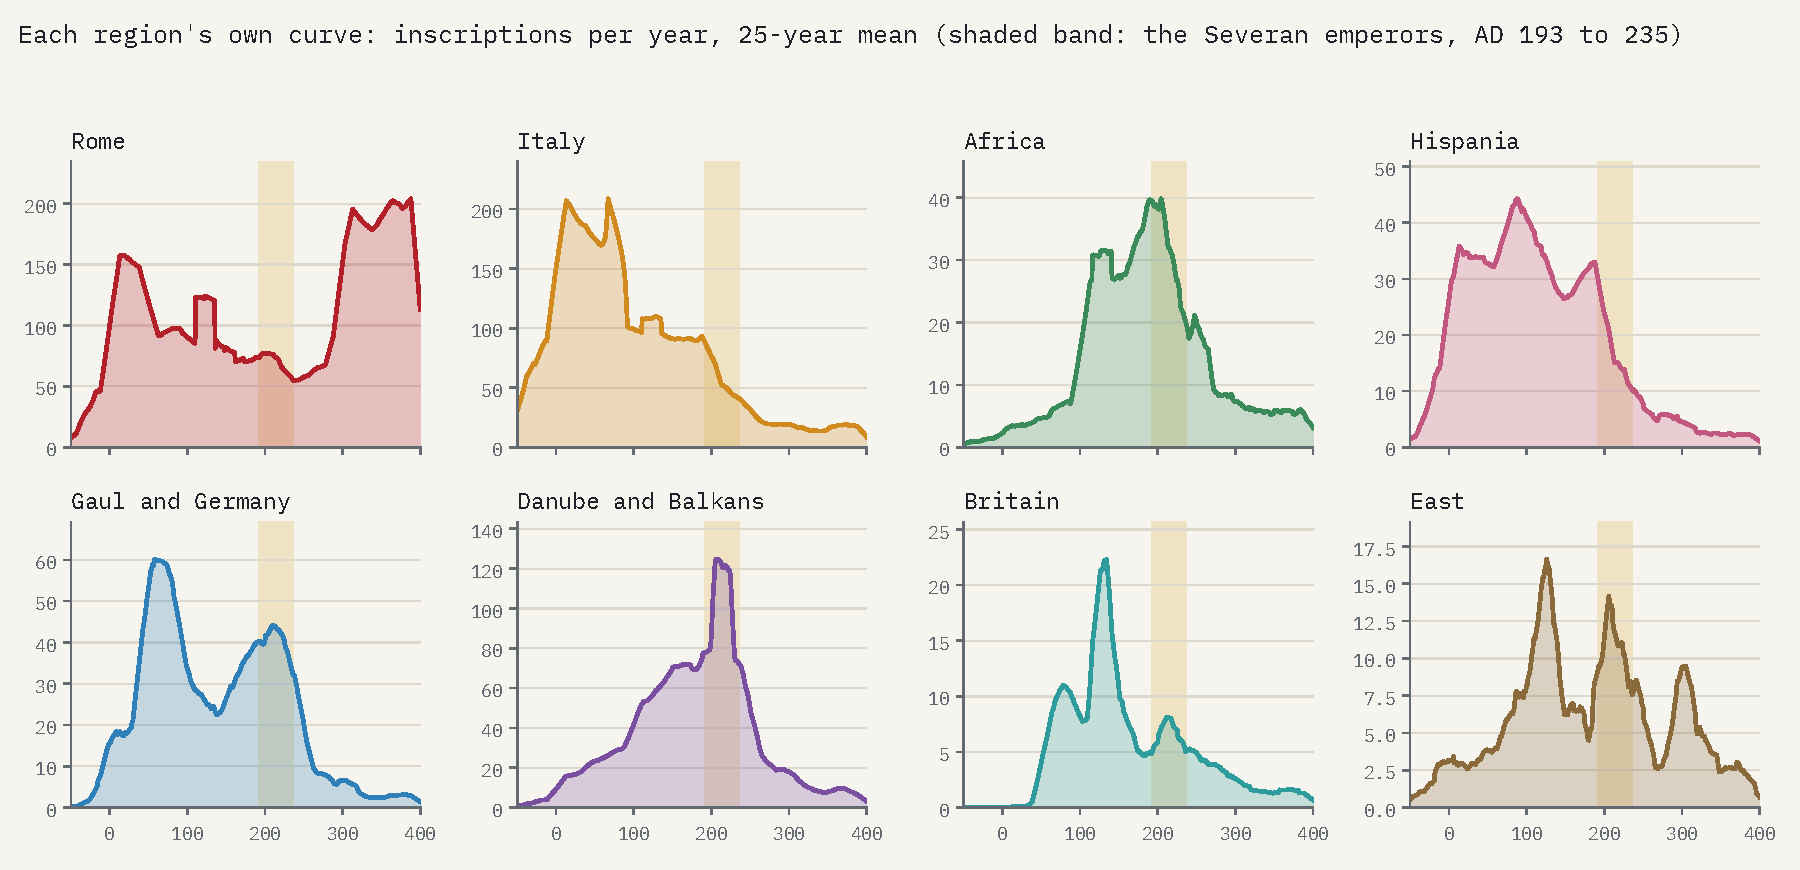
\includegraphics[width=\textwidth]{f_groups.pdf}\caption{Inscriptions per year by regional group (25-year moving mean of the aoristic sum, range 100 years or less). Each panel has its own scale.}\label{fig:groups}\end{figure}

\begin{figure}[tbp]\centering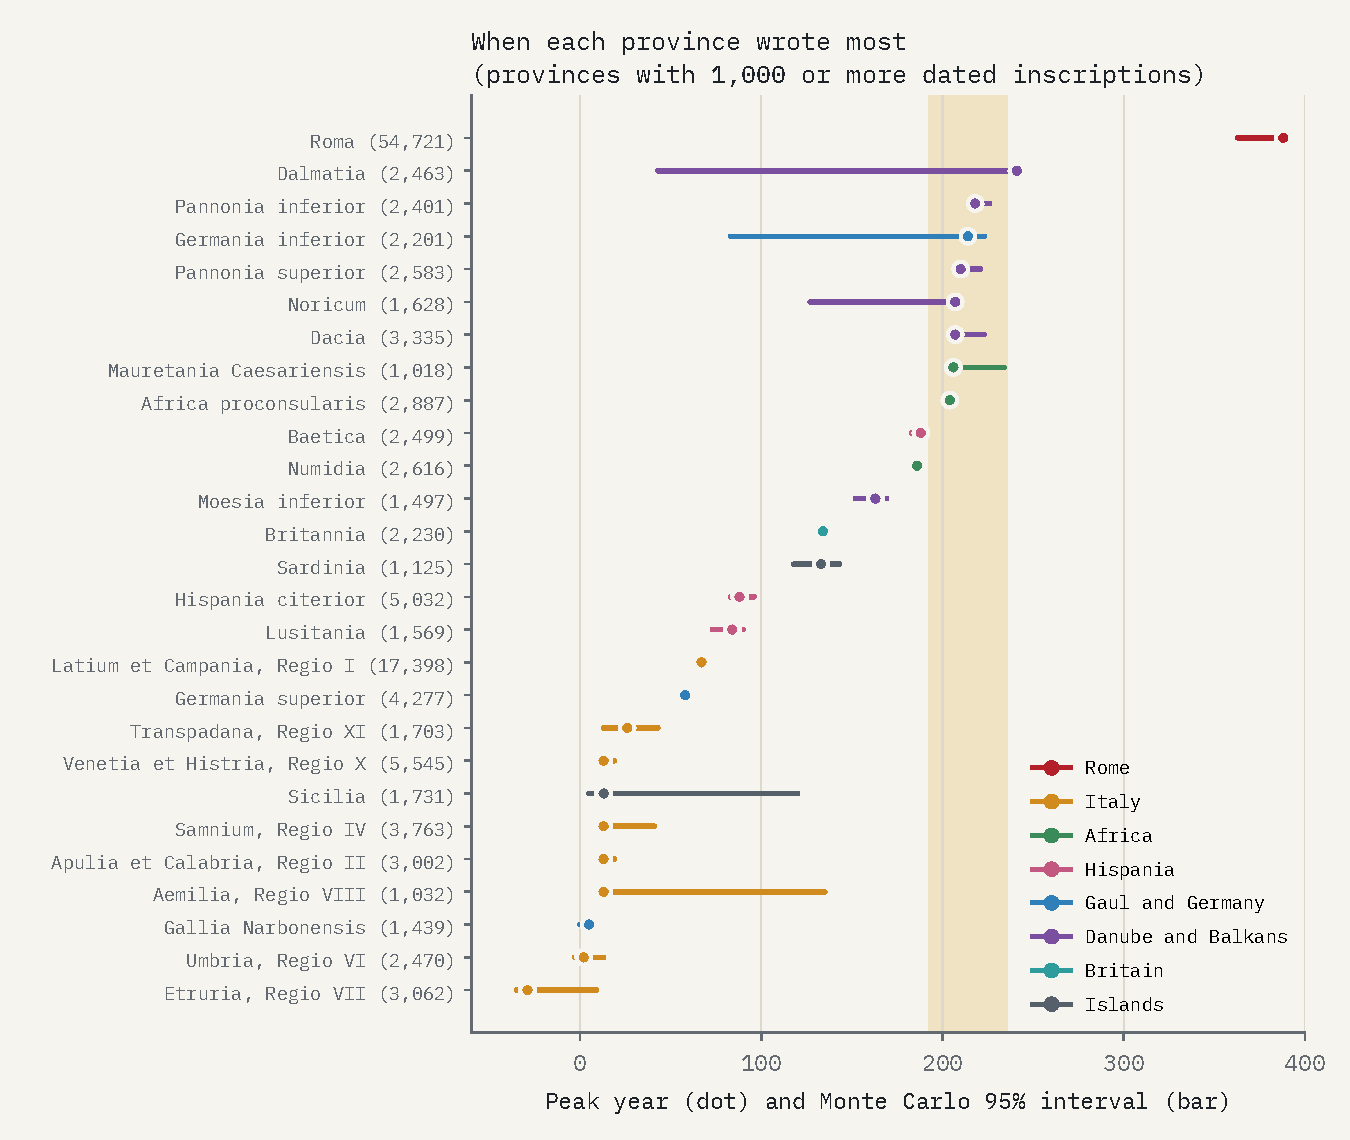
\includegraphics[width=0.86\textwidth]{f_peaks.pdf}\caption{Peak year of the 25-year moving mean by province (EDCS provinces with at least 1,000 inscriptions in the main set) with Monte Carlo 95\% intervals (200 replicates). Number of inscriptions in brackets.}\label{fig:peaks}\end{figure}

The types differ too (Table~\ref{tab:types}). Epitaphs, the largest type, peak in AD 13, driven by Italy. The public and religious types peak much later: votive inscriptions in AD 209 (interval 205 to 218), honorific ones in 205 (204 to 207) and milestones in 247 (241 to 247). Building inscriptions peak in 126. The Severan peak MacMullen saw is clearest in the inscriptions of the provinces and in dedications and honours, the kinds of text that addressed a public.

\begin{table}[tbp]\centering\small\caption{Peak year by type of inscription (LIRE type; main set) with Monte Carlo 95\% intervals (200 replicates).}\label{tab:types}\begin{tabular}{lrrr}\toprule Type & N & Peak (AD) & 95\% interval\\\midrule
Epitaphs & 79,881 & 13 & 13 to 19\\
Votive & 10,734 & 209 & 205 to 218\\
Honorific & 6,386 & 205 & 204 to 207\\
Building or dedicatory & 3,054 & 126 & 126 to 134\\
Milestones & 2,793 & 247 & 241 to 247\\
Christian (EDCS category) & 31,553 & 388 & 364 to 388\\
Not Christian & 115,885 & 68 & 13 to 72\\
\bottomrule\end{tabular}\end{table}

\begin{table}[tbp]\centering\footnotesize\caption{Peak year by EDCS province (main set, provinces with at least 1,000 inscriptions), Monte Carlo 95\% interval (200 replicates), and the ratio of the mean annual count in 193 to 235 to that in 250 to 300.}\label{tab:peaks}\begin{tabular}{llrrrr}\toprule Province & Group & N & Peak & 95\% interval & Ratio\\\midrule
Etruria, Regio VII & Italy & 3,062 & 29 BC & 35 BC to 9 & 1.9\\
Umbria, Regio VI & Italy & 2,470 & 2 & 3 BC to 13 & 1.8\\
Gallia Narbonensis & Gaul and Germany & 1,439 & 5 & 0 BC to 7 & 1.7\\
Aemilia, Regio VIII & Italy & 1,032 & 13 & 9 to 135 & 2.7\\
Apulia et Calabria, Regio II & Italy & 3,002 & 13 & 12 to 19 & 2.8\\
Samnium, Regio IV & Italy & 3,763 & 13 & 12 to 41 & 3.3\\
Sicilia & Islands & 1,731 & 13 & 5 to 120 & 2.4\\
Venetia et Histria, Regio X & Italy & 5,545 & 13 & 13 to 19 & 1.7\\
Transpadana, Regio XI & Italy & 1,703 & 26 & 13 to 43 & 1.7\\
Germania superior & Gaul and Germany & 4,277 & 58 & 58 to 60 & 7.8\\
Latium et Campania, Regio I & Italy & 17,398 & 67 & 67 to 67 & 3.9\\
Lusitania & Hispania & 1,569 & 84 & 73 to 90 & 4.8\\
Hispania citerior & Hispania & 5,032 & 88 & 83 to 96 & 1.9\\
Sardinia & Islands & 1,125 & 133 & 118 to 143 & 2.2\\
Britannia & Britain & 2,230 & 134 & 131 to 134 & 1.8\\
Moesia inferior & Danube and Balkans & 1,497 & 163 & 152 to 169 & 3.1\\
Numidia & Africa & 2,616 & 186 & 183 to 188 & 7.6\\
Baetica & Hispania & 2,499 & 188 & 183 to 188 & 5.3\\
Africa proconsularis & Africa & 2,887 & 204 & 204 to 206 & 1.5\\
Mauretania Caesariensis & Africa & 1,018 & 206 & 205 to 234 & 3.0\\
Dacia & Danube and Balkans & 3,335 & 207 & 205 to 223 & 9.4\\
Noricum & Danube and Balkans & 1,628 & 207 & 127 to 208 & 4.4\\
Pannonia superior & Danube and Balkans & 2,583 & 210 & 206 to 221 & 2.9\\
Germania inferior & Gaul and Germany & 2,201 & 214 & 83 to 223 & 6.9\\
Pannonia inferior & Danube and Balkans & 2,401 & 218 & 218 to 226 & 4.4\\
Dalmatia & Danube and Balkans & 2,463 & 241 & 43 to 244 & 1.5\\
Roma & Rome & 54,721 & 388 & 363 to 388 & 0.9\\
\bottomrule\end{tabular}\end{table}

\subsection{H2: ages at death and rounding}
The extraction gives 29,598 ages on 27,387 stones, 23\% of the 118,694 epitaphs with text: 22,812 in the \textit{vixit} form and 6,786 in the genitive form; 880 are given \textit{plus minus}. Figure~\ref{fig:ages} shows the distribution. Between 23 and 62 there are 5,020 ages ending in 0 and 3,474 ending in 5, against 1,404 per digit expected without preference: 3.6 and 2.5 times the expectation. Whipple's index is 302.6 (95\% CI 298.4 to 306.8; ABCC 49), and Myers' blended index 35.2.

\begin{figure}[tbp]\centering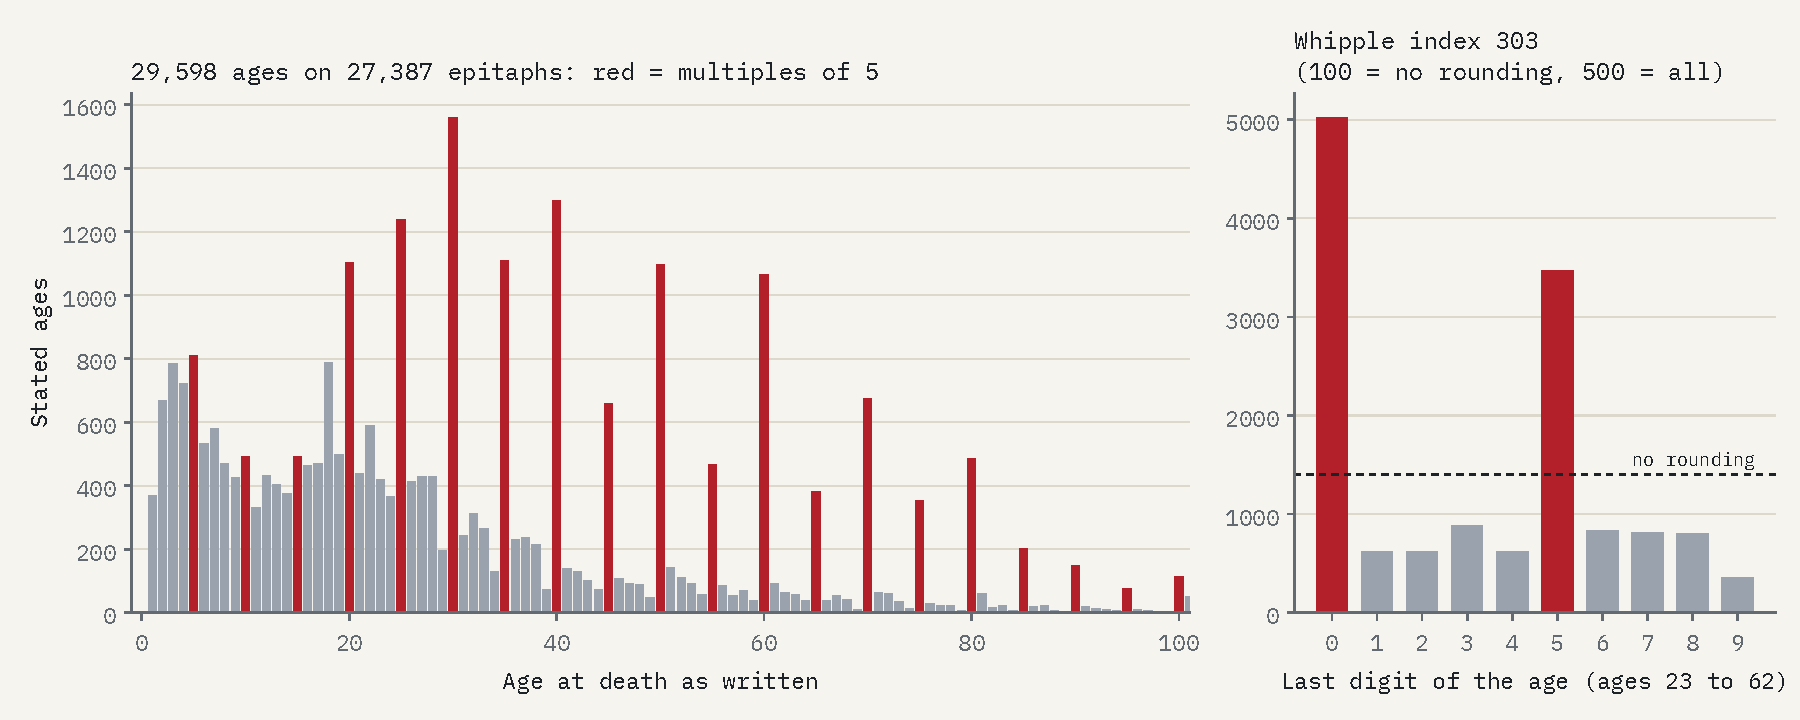
\includegraphics[width=\textwidth]{f_ages.pdf}\caption{Left: stated ages at death on epitaphs (multiples of five in red). Right: last digit of ages 23 to 62; dashed line, the count expected with no digit preference.}\label{fig:ages}\end{figure}

H2a is supported: the index is above 100 in every regional group with enough ages (Table~\ref{tab:whipple}, Figure~\ref{fig:whipple}), from 248 in Rome to 372 in the Danube and Balkan provinces. Rounding is lighter on Christian epitaphs (249), heavier in the genitive form (360) than in the \textit{vixit} form (283), and heavier on ages given \textit{plus minus} (360), as the phrase implies. By setting it rises from 251 in large cities to 362 in the countryside.

\begin{figure}[tbp]\centering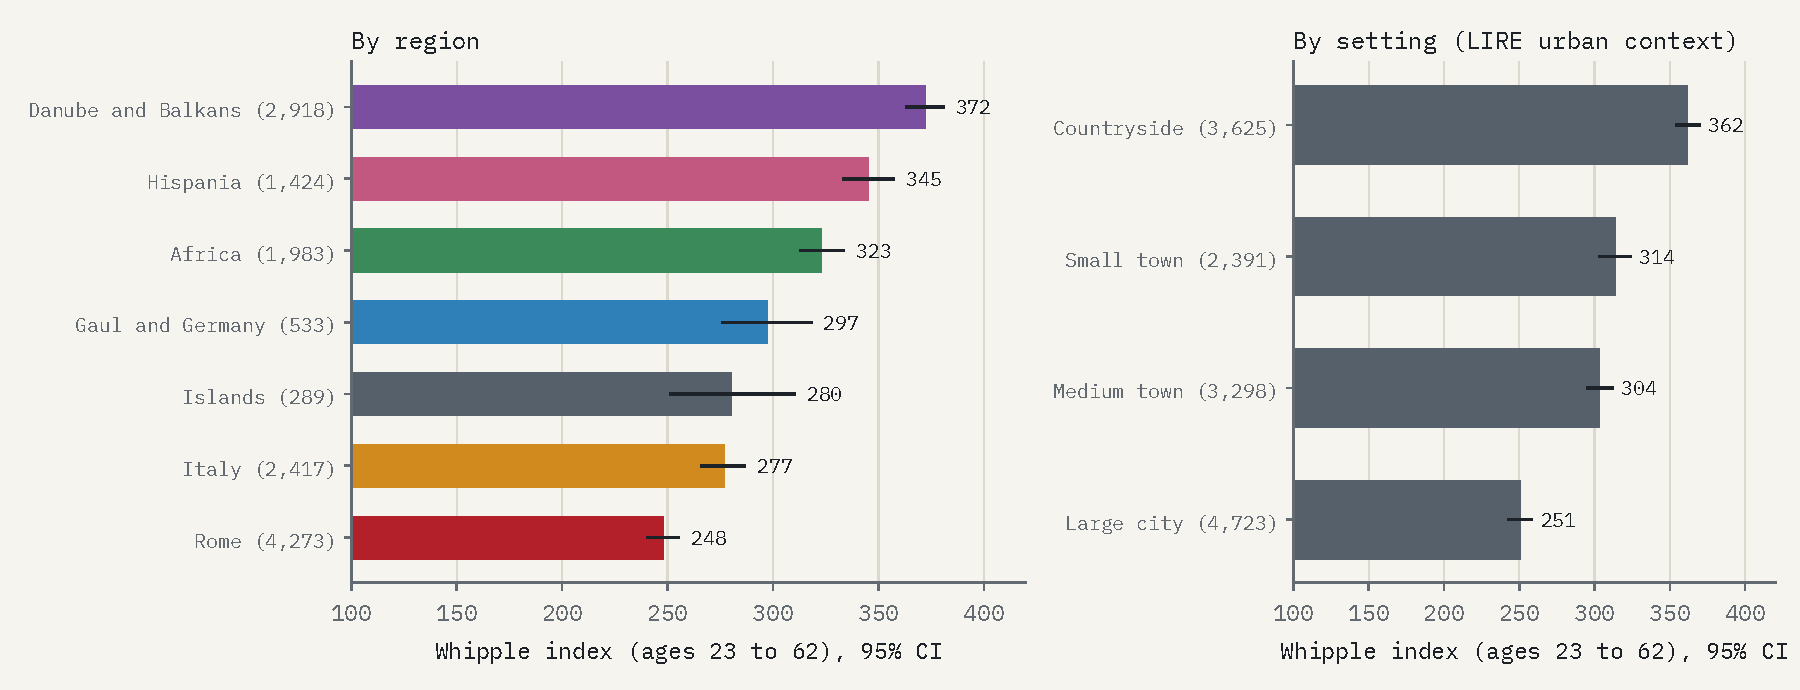
\includegraphics[width=\textwidth]{f_whipple.pdf}\caption{Whipple's index (ages 23 to 62) by regional group and by LIRE urban context, with bootstrap 95\% intervals (resampling stones). Number of ages in brackets.}\label{fig:whipple}\end{figure}

\begin{table}[tbp]\centering\small\caption{Age rounding: Whipple's index on ages 23 to 62 with bootstrap 95\% intervals (stones resampled), the ABCC index, and Myers' blended index (ages 10 to 89; groups with at least 300 ages). N: ages 23 to 62. Britain and the East have fewer than 200 ages in the range.}\label{tab:whipple}\begin{tabular}{lrrlrr}\toprule Subset & N & Whipple & 95\% CI & ABCC & Myers\\\midrule
All ages & 14,037 & 302.6 & [298.4, 306.8] & 49.4 & 35.2\\
\multicolumn{6}{l}{\textit{Regional group}}\\
\quad Rome & 4,273 & 247.8 & [240.8, 255.1] & 63.0 & 22.7\\
\quad Italy & 2,417 & 277.0 & [266.2, 286.5] & 55.8 & 28.3\\
\quad Africa & 1,983 & 323.0 & [313.1, 333.5] & 44.3 & 44.3\\
\quad Hispania & 1,424 & 345.2 & [333.4, 357.0] & 38.7 & 44.9\\
\quad Gaul and Germany & 533 & 297.4 & [276.2, 317.9] & 50.7 & 36.0\\
\quad Danube and Balkans & 2,918 & 372.3 & [363.3, 380.6] & 31.9 & 49.9\\
\quad Islands & 289 & 280.3 & [251.7, 309.9] & 54.9 & 31.5\\
\multicolumn{6}{l}{\textit{Urban context}}\\
\quad large & 4,723 & 250.7 & [243.0, 258.2] & & \\
\quad medium & 3,298 & 303.5 & [295.6, 311.7] & & \\
\quad small & 2,391 & 313.7 & [303.7, 323.6] & & \\
\quad rural & 3,625 & 361.9 & [354.3, 369.5] & & \\
\multicolumn{6}{l}{\textit{Form and status}}\\
\quad vixit form & 10,436 & 282.6 & [278.5, 287.5] & & \\
\quad genitive form (annorum) & 3,601 & 360.3 & [353.5, 368.6] & & \\
\quad given plus minus & 541 & 359.5 & [340.0, 380.4] & & \\
\quad Christian & 2,335 & 249.3 & [239.4, 260.1] & & \\
\quad not Christian & 11,702 & 313.2 & [309.1, 317.8] & & \\
\bottomrule\end{tabular}\end{table}

The planned model (Table~\ref{tab:model}) separates these factors. H2b is not supported: holding setting, age band and Christian status fixed, the odds that an African age is a multiple of five are 1.22 times those in Rome (95\% CI 0.88 to 1.68, $N = 14,036$ ages, 2,031 findspots). The raw African excess reflects the setting and the ages of African epitaphs: among ages 23 to 62, 40\% of African ages are from rural contexts and 9\% from large cities, against none rural in Rome, and their mean is 41.9 against 35.4. The regions with a significant excess over Rome are the Danube and Balkan provinces (odds ratio 2.02, 1.41 to 2.90) and Hispania (1.48, 1.04 to 2.09). H2c is supported in the main model: rural ages are more often rounded than those in large cities (odds ratio 1.50, 1.09 to 2.07); medium and small towns do not differ from large cities. H2d is supported: against ages 23 to 32, the odds ratios are 1.71, 2.12 and 2.48 for the three older bands. The full coefficients are in Appendix Table~\ref{tab:modelfull}. Christian epitaphs round less (odds ratio 0.80, 0.69 to 0.93).

\begin{table}[tbp]\centering\small\caption{The planned model (H2b to H2d): logistic regression of whether a stated age (23 to 62) is a multiple of five. Odds ratios with 95\% intervals from standard errors clustered by findspot. N = 14,036 ages, 2,031 findspots.}\label{tab:model}\begin{tabular}{lrlr}\toprule Term & Odds ratio & 95\% CI & $p$\\\midrule
\multicolumn{4}{l}{\textit{Regional group (reference: Rome)}}\\
\quad Italy & 1.00 & [0.69, 1.44] & 0.989\\
\quad Africa & 1.22 & [0.88, 1.68] & 0.233\\
\quad Hispania & 1.48 & [1.04, 2.09] & 0.029\\
\quad Gaul and Germany & 1.17 & [0.77, 1.79] & 0.457\\
\quad Danube and Balkans & 2.02 & [1.41, 2.90] & 0.000\\
\quad Britain & 1.16 & [0.68, 1.98] & 0.592\\
\quad East & 0.83 & [0.49, 1.39] & 0.473\\
\quad Islands & 0.89 & [0.54, 1.47] & 0.651\\
\multicolumn{4}{l}{\textit{Urban context (reference: large)}}\\
\quad medium & 1.05 & [0.73, 1.51] & 0.805\\
\quad small & 1.11 & [0.78, 1.58] & 0.562\\
\quad rural & 1.50 & [1.09, 2.07] & 0.014\\
\multicolumn{4}{l}{\textit{Age band (reference: 23 to 32)}}\\
\quad 33 to 42 & 1.71 & [1.55, 1.88] & 0.000\\
\quad 43 to 52 & 2.12 & [1.90, 2.36] & 0.000\\
\quad 53 to 62 & 2.48 & [2.20, 2.78] & 0.000\\
Christian inscription & 0.80 & [0.69, 0.93] & 0.005\\
\bottomrule\end{tabular}\end{table}

Exploratory, by period (dated stones, range 100 years or less, by midpoint), the index is 321 for AD 51 to 150, 299 for 151 to 250 and 230 for 251 to 350, the lower late value reflecting the weight of Christian epitaphs from Rome in that period.

\textit{Why tombstones are not life tables.} Table~\ref{tab:hopkins} and Figure~\ref{fig:hopkins} repeat Hopkins's argument with the full corpus. The mean stated age at death is 23.2 in Rome and 47.8 in Africa. Only 7.1\% of African ages are under ten, against 28.4\% in Rome and 18.1\% overall, whereas in any population with Roman levels of mortality a large share of all deaths were of young children \citep{hopkins1966,scheidel2001}. 246 stated ages are 100 or more, 154 of them in Africa, and 26\% of African ages are 70 or more. Differences of this size between regions reflect who was commemorated and how ages were recorded, not mortality.

\begin{figure}[tbp]\centering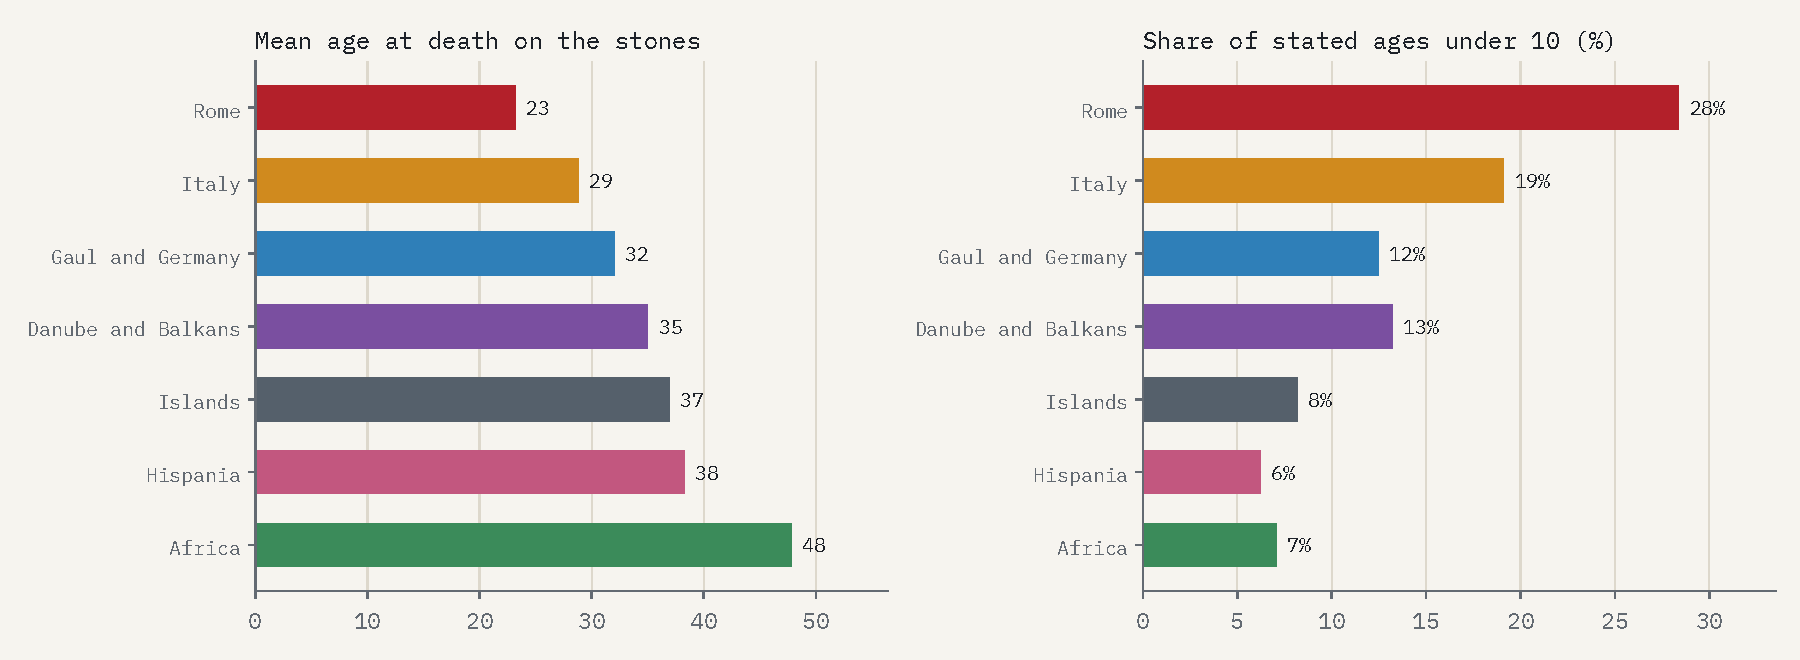
\includegraphics[width=\textwidth]{f_hopkins.pdf}\caption{Mean stated age at death and share of stated ages under ten, by regional group.}\label{fig:hopkins}\end{figure}

\begin{table}[tbp]\centering\small\caption{Stated ages at death by regional group (groups with at least 300 ages): mean, median, share under ten, share of 70 or more, and number of ages of 100 or more.}\label{tab:hopkins}\begin{tabular}{lrrrrrr}\toprule Group & Ages & Mean & Median & Under 10 (\%) & 70+ (\%) & 100+\\\midrule
Rome & 10,583 & 23.2 & 20 & 28.4 & 3.2 & 17\\
Italy & 5,409 & 28.8 & 24 & 19.1 & 6.4 & 11\\
Africa & 4,086 & 47.8 & 45 & 7.1 & 26.1 & 154\\
Hispania & 2,578 & 38.3 & 33 & 6.2 & 12.6 & 16\\
Gaul and Germany & 857 & 32.1 & 30 & 12.5 & 5.3 & 2\\
Danube and Balkans & 5,256 & 35.0 & 30 & 13.2 & 9.6 & 41\\
Islands & 514 & 36.9 & 35 & 8.2 & 9.5 & 4\\
\midrule All & 29,598 & 31.6 & 27 & 18.1 & 9.1 & 246\\
\bottomrule\end{tabular}\end{table}

\subsection{H3: soldiers' origins}
Of 19,484 military inscriptions (and 503 diplomas, analysed apart), 865 (4.4\%) state an origin that could be placed: 510 at a town and 355 at a people or region; 28 more were ambiguous and dropped. Only 13 diplomas gave a mapped origin. This is above the planned threshold of 300, so Part~3 is reported as planned. Figure~\ref{fig:soldiers} maps the journeys. The median distance from origin to stone is 674~km; 68\% are over 500~km and 2.8\% under 50~km. 36\% of the stones stand in the city of Rome. The commonest origins are Pannonia, the Bessi of Thrace, Verona, Syria and Egypt (Table~\ref{tab:routes}). The commonest routes run from Pannonia, Syria and the Batavian homeland to Rome and from Egypt, Thrace and Cilicia to Campania (the fleet at Misenum), consistent with the empire-wide recruitment of the guard units and fleets; northern Italian towns such as Verona and Bononia appear mainly on earlier stones.

\begin{figure}[tbp]\centering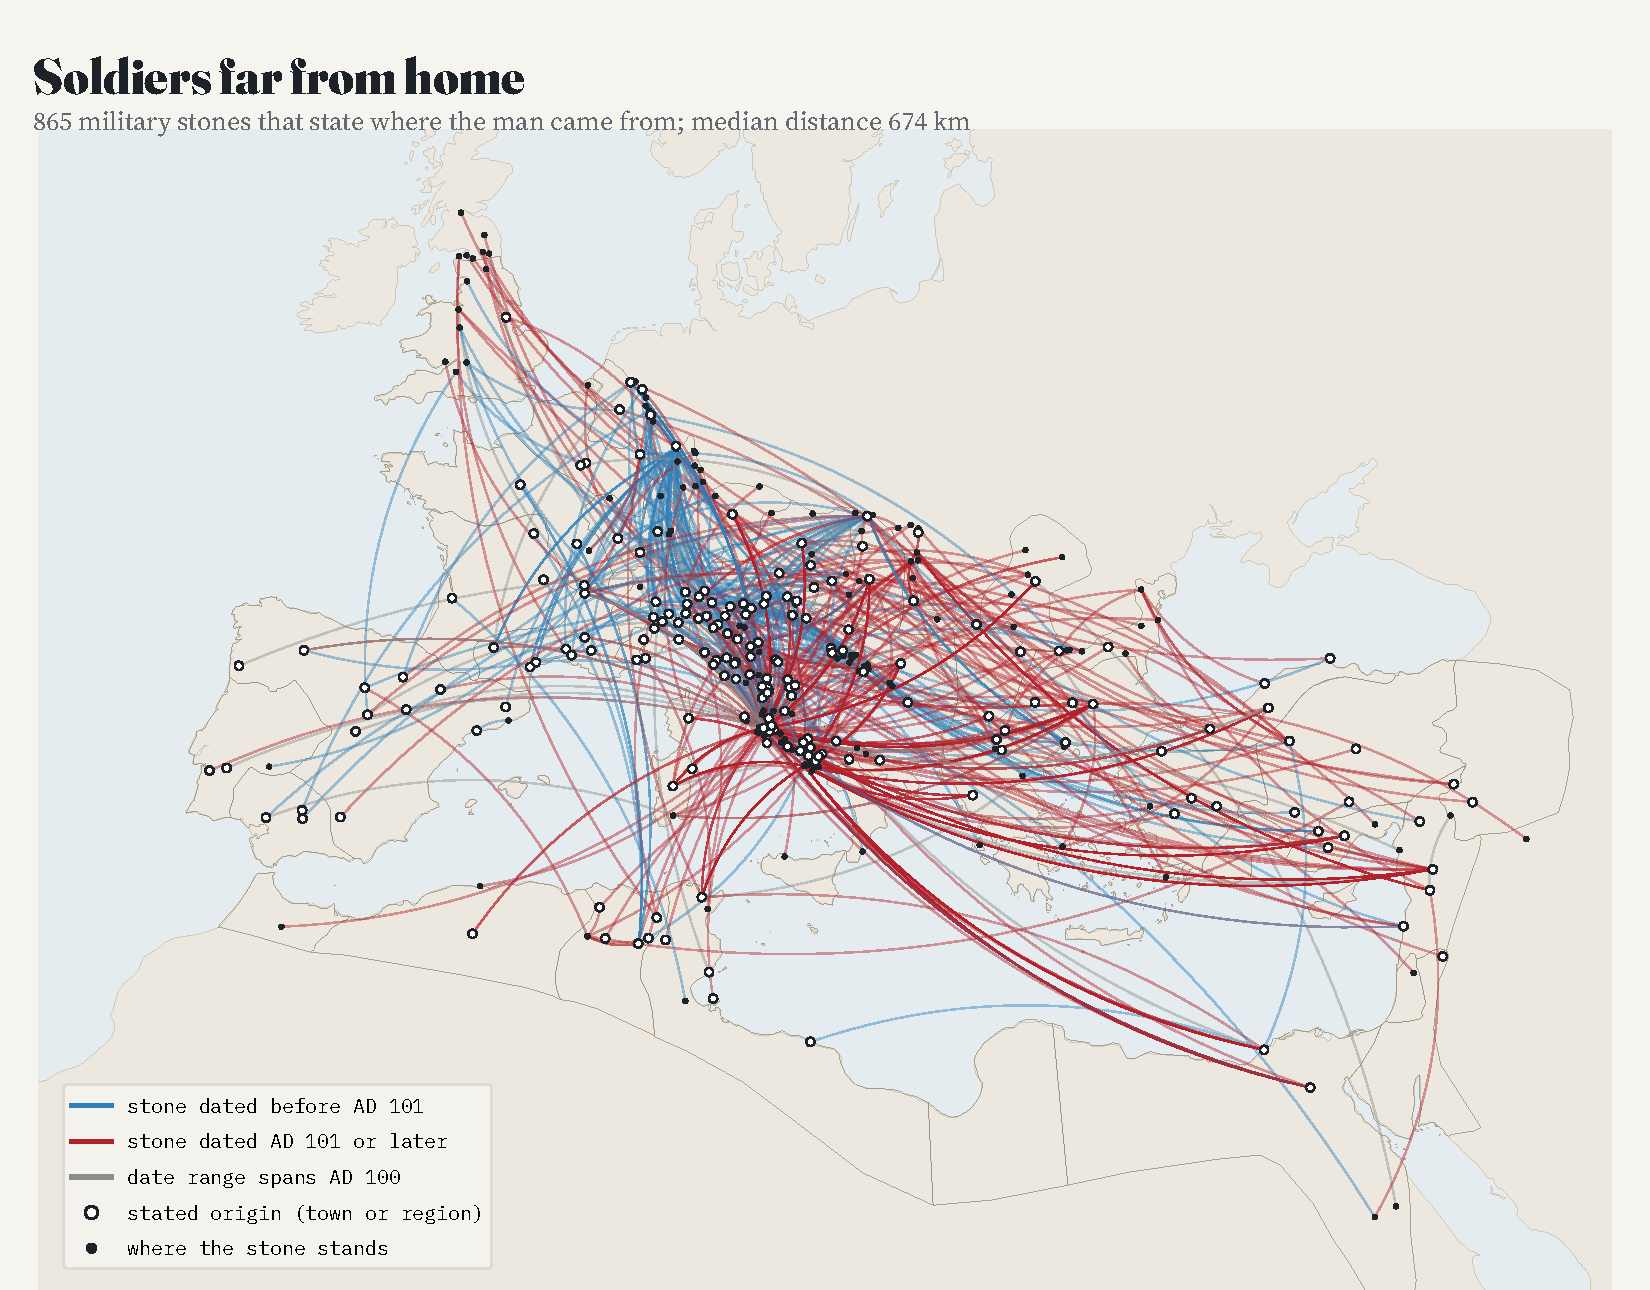
\includegraphics[width=\textwidth]{f_soldiers.pdf}\caption{Military stones with a stated and mapped origin: lines from origin (open circle; a town or a point for a people or region) to findspot (dot). Blue: stones dated before AD 101; red: AD 101 or later; grey: date range spans AD 100.}\label{fig:soldiers}\end{figure}

H3 is not supported (Table~\ref{tab:h3}). Among 768 stones that can be placed wholly before AD 101 (266) or wholly in 101 to 300 (502), the median distance is 545~km for the earlier and 750~km for the later stones. The median regression gives a ratio of 1.37 (cluster bootstrap 95\% interval 1.22 to 1.90, 179 findspots): later stones name homes further away, not nearer. Among origins given as towns the ratio is 1.03 (0.81 to 1.65), no change in either direction.

\begin{table}[tbp]\centering\small\caption{H3. Median distance (km) from stated origin to findspot for military stones dated wholly before AD 101 (earlier) and wholly in 101 to 300 (later), and the ratio of medians from a median regression of log distance, with cluster bootstrap 95\% intervals (findspots resampled). H3 predicted a ratio below 1.}\label{tab:h3}\begin{tabular}{lrrrrl}\toprule Specification & N earlier / later & Earlier & Later & Ratio & 95\% CI\\\midrule
Main: all mapped soldier stones & 266 / 502 & 545 & 750 & 1.37 & [1.22, 1.90]\\
City origins only & 237 / 198 & 538 & 563 & 1.03 & [0.81, 1.65]\\
Excluding findspots in Rome & 216 / 294 & 569 & 966 & 1.70 & [1.26, 1.95]\\
Excluding Rome and Italy & 174 / 137 & 642 & 915 & 1.42 & [1.02, 2.04]\\
Date range 100 years or less & 266 / 434 & 545 & 714 & 1.30 & [1.19, 1.86]\\
\bottomrule\end{tabular}\end{table}

\section{Robustness}\label{sec:robust}
\textit{The habit.} The ratio of 193 to 235 over 250 to 300 lies between 1.83 (all dated) and 2.20 (main) across the four dating sets, and the empire-wide peak lies in the first or early second century in all of them (Table~\ref{tab:habit}). The Monte Carlo intervals for the ratio are narrow because the corpus is large; the uncertainty that matters is not sampling but the editors' dating conventions (Section~\ref{sec:disc}).

\textit{Age rounding.} Table~\ref{tab:robust} and Figure~\ref{fig:robust} show the planned checks. The Africa contrast stays near 1 with intervals including 1 in every check. The rural contrast keeps an odds ratio between about 1.3 and 1.8 in every check, but its interval includes 1 when only the \textit{vixit} form is used (odds ratio 1.29, 0.92 to 1.82). The rural result is therefore suggestive rather than robust. The age gradient is large in every specification.

\textit{Soldiers.} The later-period ratio is above 1 in the main specification, when findspots in Rome are excluded (1.70), when Rome and Italy are excluded (1.42), and with date ranges of 100 years or less (1.30); it is 1.03 for town origins only. No specification shows origins moving closer.

\begin{figure}[tbp]\centering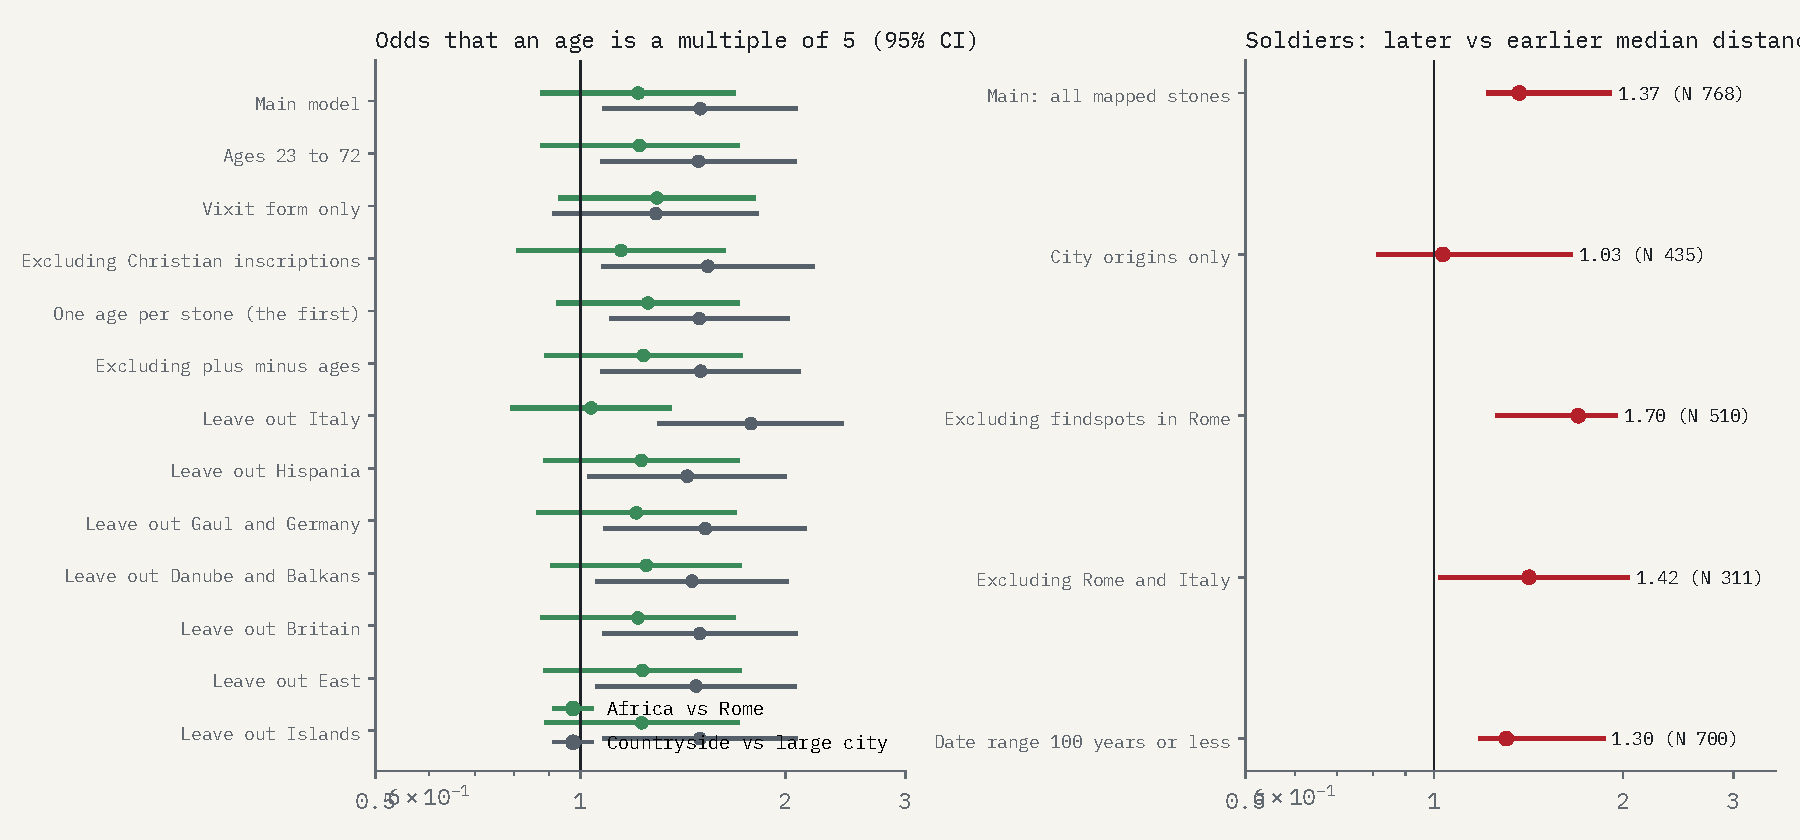
\includegraphics[width=\textwidth]{f_robust.pdf}\caption{Left: odds ratios that an age is a multiple of five, Africa against Rome and countryside against large cities, across the planned checks. Right: ratio of median origin-to-stone distance, later (101 to 300) over earlier (before 101) stones, across the planned checks. 95\% intervals.}\label{fig:robust}\end{figure}

\begin{table}[tbp]\centering\small\caption{Planned robustness checks for the age model: odds ratios (95\% CI) for Africa against Rome and rural against large urban contexts.}\label{tab:robust}\begin{tabular}{lrll}\toprule Specification & N & Africa vs Rome & Rural vs large\\\midrule
Main model & 14,036 & 1.22 [0.88, 1.68] & 1.50 [1.09, 2.07]\\
Ages 23 to 72 & 15,460 & 1.22 [0.88, 1.70] & 1.49 [1.08, 2.06]\\
Vixit form only & 10,435 & 1.30 [0.93, 1.80] & 1.29 [0.92, 1.82]\\
Excluding Christian inscriptions & 11,701 & 1.15 [0.81, 1.62] & 1.54 [1.08, 2.19]\\
One age per stone (the first) & 13,147 & 1.26 [0.93, 1.70] & 1.50 [1.11, 2.01]\\
Excluding plus minus ages & 13,495 & 1.24 [0.89, 1.72] & 1.50 [1.08, 2.09]\\
Leave out Italy & 11,619 & 1.04 [0.80, 1.35] & 1.78 [1.31, 2.42]\\
Leave out Hispania & 12,612 & 1.23 [0.89, 1.70] & 1.44 [1.03, 1.99]\\
Leave out Gaul and Germany & 13,503 & 1.21 [0.87, 1.68] & 1.53 [1.09, 2.14]\\
Leave out Danube and Balkans & 11,118 & 1.25 [0.91, 1.71] & 1.46 [1.06, 2.01]\\
Leave out Britain & 13,906 & 1.22 [0.88, 1.68] & 1.50 [1.08, 2.07]\\
Leave out East & 13,967 & 1.23 [0.89, 1.71] & 1.48 [1.06, 2.06]\\
Leave out Islands & 13,747 & 1.23 [0.89, 1.70] & 1.50 [1.09, 2.07]\\
\bottomrule\end{tabular}\end{table}

\section{Discussion}\label{sec:disc}
\subsection{The habit was provincial and public}
The collapse after the Severans is the most robust result here: whichever dating set is used, the empire wrote at most 55\% as much per year in the second half of the third century as under the Severans. But the corpus as a whole peaks in the first century, because Rome and Italy, with most of the inscriptions, inscribed most in the first century AD and declined slowly afterwards. MacMullen's Severan peak is a feature of the provinces (Africa, the Danube, Dacia, Lower Germany, Baetica) and of public and religious texts: votive and honorific inscriptions and milestones. This fits the arguments of \citet{meyer1990} and \citet{woolf1996}, in which the habit spread with Roman status and Roman society into the provinces, and it suggests that ``the epigraphic habit'' is better described as a set of regional habits with different timing than as one empire-wide curve. Italy's early peak may partly be a dating effect: epitaphs dated by formula and letter forms receive conventional ranges, and those ranges shape the curve. That caveat applies to every province, and the provincial Severan peaks are clearest in votive and honorific inscriptions.

\subsection{Rounding measures commemoration, not only numeracy}
Age rounding on Latin epitaphs is universal and heavy, as \citet{duncanjones1977} found. It grows with age, as in modern populations with limited records, and it is lighter in large cities. But the region contrast that has carried most interpretive weight, Africa against Rome, does not survive holding setting and age fixed. The rounding index of a region partly reflects the kind of commemoration typical there: in Africa, stones of the countryside that give old, often very old, ages; in Rome, urban epitaphs, many of children and the young. Read as a numeracy index in the manner of \citet{ahearn2009}, these figures measure the numeracy of commemorative practice, which may differ from that of the population. The rural excess is suggestive, and the lighter rounding on Christian epitaphs fits the same reading.

\subsection{The stones that name a home are a biased sample}
The soldiers' result runs against the classic finding of increasingly local recruitment. The data do not overturn \citet{forni1953} or \citet{mann1983}: those studies classify origins of all recruits whose origin is known, including those named by tribe in lists and diplomas, and their conclusion concerns the legions, while a large part of this sample is the guard and the fleets. What the result shows is that stones stating an origin are selected: a soldier buried near his birthplace had little reason to name it, while a Thracian at Misenum or a Pannonian in the horse guard at Rome named his people. As recruitment became local, fewer stones would state an origin at all, and those that did would be the far-travelled. The longer later distances come from the mix of forms: 61\% of the later stones give a people or region (such as \textit{natione Bessus}) against 11\% of the earlier ones, and 73\% of the later stones stand in Rome or Italy against 35\%. Among town origins there is no trend. The question of local recruitment cannot be answered from stated origins on stones alone.

\subsection{Limitations}
Four limitations apply throughout. First, survival, discovery, publication and digitisation are uneven: Rome, Italy and intensively studied provinces are over-represented, Greek inscriptions are absent and many findspots are of reuse, not of making. Second, dates are editors' ranges, some conventional and some type-based (Christian epitaphs are dated late because they are Christian); aoristic and Monte Carlo methods spread the uncertainty but cannot correct biased conventions. Third, ages and origins are read with explicit rules that miss forms outside them (ages in words; origins without a keyword) and make a small number of errors, measured in the validation samples. Fourth, all three analyses are observational. They describe patterns in what was written and cannot by themselves identify why it was written.

\section{Conclusion}\label{sec:conc}
A harmonised corpus of 203,466 Latin inscriptions confirms the scale of the third-century collapse of the epigraphic habit, places its Severan peak in the provinces and in public and religious inscriptions rather than in the corpus as a whole, shows that ages on tombstones were rounded everywhere, more at older ages and probably more in the countryside, without a distinct African excess once those factors are held fixed, and finds that soldiers who named their homes did not name nearer ones over time, a sign of selection rather than of recruitment. Each test was fixed in advance, three of the six planned hypotheses (H1a, H2b and H3) failed by their own criteria, and the rules, samples and code are released so that others can change them and see what follows.

\section*{Data availability}
Data and code: Zenodo DOI https://doi.org/10.5281/zenodo.24114976. The derived tables (one row per inscription without texts, the extracted ages, the soldiers' origins, the aoristic curves and every number in this paper) are released under CC BY 4.0, including the province outlines derived from DARE (CC BY 4.0). LIRE v2.1 is available from Zenodo (doi:10.5281/zenodo.7577788) under CC BY 4.0. An interactive map is at \url{https://maps.tristanhotham.com/roman-inscriptions/}.

\section*{AI statement}
I wrote the text, with drafting and editing assistance from Claude (Anthropic), which also helped prepare the analysis code. I reviewed and checked all text and results.

\begin{thebibliography}{99}
\bibitem[A'Hearn et~al.(2009)]{ahearn2009} A'Hearn, B., Baten, J. and Crayen, D. (2009) Quantifying quantitative literacy: age heaping and the history of human capital. \textit{Journal of Economic History} 69(3): 783-808. doi:10.1017/S0022050709001120.
\bibitem[{\AA}hlfeldt(2013)]{ahlfeldt2013} {\AA}hlfeldt, J. (2013) \textit{Digital Atlas of the Roman Empire}. Web publication. Lund: Lund University. \url{http://dare.ht.lu.se}.
\bibitem[Baxter and Cool(2016)]{baxtercool2016} Baxter, M. J. and Cool, H. E. M. (2016) Reinventing the wheel? Modelling temporal uncertainty with applications to brooch distributions in Roman Britain. \textit{Journal of Archaeological Science} 66: 120-127. doi:10.1016/j.jas.2015.12.007.
\bibitem[Beltr{\'a}n Lloris(2014)]{beltran2014} Beltr{\'a}n Lloris, F. (2014) The ``epigraphic habit'' in the Roman world. In C. Bruun and J. Edmondson (eds), \textit{The Oxford Handbook of Roman Epigraphy}, chapter 8 (from p. 131). New York: Oxford University Press.
\bibitem[Bodel(2014)]{bodel2014} Bodel, J. (2014) Inscriptions and literacy. In Bruun and Edmondson (2014), chapter 34 (from p. 745).
\bibitem[Bruun and Edmondson(2014)]{bruun2014} Bruun, C. and Edmondson, J. (eds) (2014) \textit{The Oxford Handbook of Roman Epigraphy}. New York: Oxford University Press.
\bibitem[Clauss et~al.(2007-)]{edcs} Clauss, M. et al. (eds) (2007-) \textit{Epigraphik-Datenbank Clauss/Slaby} (EDCS). Eichst{\"a}tt. \url{http://www.manfredclauss.de/}.
\bibitem[Alf{\"o}ldy and Witschel(1997-)]{edh} Alf{\"o}ldy, G. and Witschel, C. (eds) (1997-) \textit{Epigraphic Database Heidelberg} (EDH). Heidelberg. \url{https://edh.ub.uni-heidelberg.de/}.
\bibitem[Crema(2012)]{crema2012} Crema, E. R. (2012) Modelling temporal uncertainty in archaeological analysis. \textit{Journal of Archaeological Method and Theory} 19(3): 440-461. doi:10.1007/s10816-011-9122-3.
\bibitem[Duncan-Jones(1977)]{duncanjones1977} Duncan-Jones, R. P. (1977) Age-rounding, illiteracy and social differentiation in the Roman Empire. \textit{Chiron} 7: 333-354. doi:10.34780/hsl9-u821.
\bibitem[Forni(1953)]{forni1953} Forni, G. (1953) \textit{Il reclutamento delle legioni da Augusto a Diocleziano}. Milano and Roma: Fratelli Bocca.
\bibitem[Frier(1982)]{frier1982} Frier, B. W. (1982) Roman life expectancy: Ulpian's evidence. \textit{Harvard Studies in Classical Philology} 86: 213-251.
\bibitem[Frier(1983)]{frier1983} Frier, B. W. (1983) Roman life expectancy: the Pannonian evidence. \textit{Phoenix} 37: 328-344.
\bibitem[Hanson(2016)]{hanson2016} Hanson, J. W. (2016) \textit{An Urban Geography of the Roman World, 100 BC to AD 300}. Archaeopress Roman Archaeology 18. Oxford: Archaeopress.
\bibitem[Haynes(2013)]{haynes2013} Haynes, I. (2013) \textit{Blood of the Provinces: The Roman Auxilia and the Making of Provincial Society from Augustus to the Severans}. Oxford: Oxford University Press. doi:10.1093/acprof:oso/9780199655342.001.0001.
\bibitem[He{\v r}m{\'a}nkov{\'a} et~al.(2021)]{hermankova2021} He{\v r}m{\'a}nkov{\'a}, P., Ka{\v s}e, V. and Sobotkov{\'a}, A. (2021) Inscriptions as data: digital epigraphy in macro-historical perspective. \textit{Journal of Digital History} 1(1): 99-141. doi:10.1515/jdh-2021-1004.
\bibitem[Hopkins(1966)]{hopkins1966} Hopkins, K. (1966) On the probable age structure of the Roman population. \textit{Population Studies} 20: 245-264.
\bibitem[Johnson(2004)]{johnson2004} Johnson, I. (2004) Aoristic analysis: seeds of a new approach to mapping archaeological distributions through time. In K. F. Ausserer, W. B{\"o}rner, M. Goriany and L. Karlhuber-V{\"o}ckl (eds), \textit{Enter the Past: The E-way into the Four Dimensions of Cultural Heritage}, 448-452. BAR International Series 1227. Oxford: Archaeopress.
\bibitem[Ka{\v s}e et~al.(2021)]{kase2021classifying} Ka{\v s}e, V., He{\v r}m{\'a}nkov{\'a}, P. and Sobotkov{\'a}, A. (2021) Classifying Latin inscriptions of the Roman Empire: a machine-learning approach. In \textit{Proceedings of the Conference on Computational Humanities Research 2021}, 123-135. CEUR Workshop Proceedings.
\bibitem[Ka{\v s}e et~al.(2022)]{kase2022division} Ka{\v s}e, V., He{\v r}m{\'a}nkov{\'a}, P. and Sobotkov{\'a}, A. (2022) Division of labor, specialization and diversity in the ancient Roman cities: a quantitative approach to Latin epigraphy. \textit{PLoS ONE} 17(6): e0269869. doi:10.1371/journal.pone.0269869.
\bibitem[Ka{\v s}e et~al.(2023)]{kase2023lire} Ka{\v s}e, V., He{\v r}m{\'a}nkov{\'a}, P. and Sobotkov{\'a}, A. (2023) \textit{LIRE (Latin Inscriptions of the Roman Empire)}, version 2.1. Dataset. Aarhus University (SDAM project). Zenodo. doi:10.5281/zenodo.7577788.
\bibitem[Kolb(2014)]{kolb2014} Kolb, A. (2014) Communications and mobility in the Roman Empire. In Bruun and Edmondson (2014), chapter 30 (from p. 649).
\bibitem[MacMullen(1982)]{macmullen1982} MacMullen, R. (1982) The epigraphic habit in the Roman Empire. \textit{American Journal of Philology} 103: 233-246.
\bibitem[Mann(1983)]{mann1983} Mann, J. C. (1983) \textit{Legionary Recruitment and Veteran Settlement during the Principate}, ed. M. M. Roxan. Institute of Archaeology Occasional Publication 7. London: Institute of Archaeology.
\bibitem[Mazzoleni(2014)]{mazzoleni2014} Mazzoleni, D. (2014) The rise of Christianity. In Bruun and Edmondson (2014), chapter 21 (from p. 445).
\bibitem[Meyer(1990)]{meyer1990} Meyer, E. A. (1990) Explaining the epigraphic habit in the Roman Empire: the evidence of epitaphs. \textit{Journal of Roman Studies} 80: 74-96. doi:10.2307/300281.
\bibitem[Mrozek(1973)]{mrozek1973} Mrozek, S. (1973) A propos de la r{\'e}partition chronologique des inscriptions latines dans le Haut-Empire. \textit{Epigraphica} 35: 113-118.
\bibitem[Myers(1940)]{myers1940} Myers, R. J. (1940) Errors and bias in the reporting of ages in census data. \textit{Transactions of the Actuarial Society of America} 41: 395-415.
\bibitem[Noy(2000)]{noy2000} Noy, D. (2000) \textit{Foreigners at Rome: Citizens and Strangers}. London: Duckworth with the Classical Press of Wales.
\bibitem[Palmisano et~al.(2017)]{palmisano2017} Palmisano, A., Bevan, A. and Shennan, S. (2017) Comparing archaeological proxies for long-term population patterns: an example from central Italy. \textit{Journal of Archaeological Science} 87: 59-72. doi:10.1016/j.jas.2017.10.001.
\bibitem[Parkin(1992)]{parkin1992} Parkin, T. G. (1992) \textit{Demography and Roman Society}. Baltimore: Johns Hopkins University Press.
\bibitem[Ratcliffe(2000)]{ratcliffe2000} Ratcliffe, J. H. (2000) Aoristic analysis: the spatial interpretation of unspecific temporal events. \textit{International Journal of Geographical Information Science} 14(7): 669-679. doi:10.1080/136588100424963.
\bibitem[Saller and Shaw(1984)]{sallershaw1984} Saller, R. P. and Shaw, B. D. (1984) Tombstones and Roman family relations in the Principate: civilians, soldiers and slaves. \textit{Journal of Roman Studies} 74: 124-156. doi:10.2307/299012.
\bibitem[Scheidel(1996)]{scheidel1996} Scheidel, W. (1996) \textit{Measuring Sex, Age and Death in the Roman Empire: Explorations in Ancient Demography}. Journal of Roman Archaeology Supplementary Series 21. Ann Arbor: JRA.
\bibitem[Scheidel(2001)]{scheidel2001} Scheidel, W. (2001) Roman age structure: evidence and models. \textit{Journal of Roman Studies} 91: 1-26. doi:10.2307/3184767.
\bibitem[Speidel(2014)]{speidel2014} Speidel, M. A. (2014) The Roman army. In Bruun and Edmondson (2014), chapter 16 (from p. 319).
\bibitem[Tacoma(2016)]{tacoma2016} Tacoma, L. E. (2016) \textit{Moving Romans: Migration to Rome in the Principate}. Oxford: Oxford University Press.
\bibitem[Woolf(1996)]{woolf1996} Woolf, G. (1996) Monumental writing and the expansion of Roman society in the early Empire. \textit{Journal of Roman Studies} 86: 22-39.
\end{thebibliography}

\appendix
\section{Supplementary tables}
\begin{table}[tbp]\centering\footnotesize\caption{The ten commonest stated origins on military stones and the commonest origin to findspot-province routes.}\label{tab:routes}\begin{tabular}{lrlr}\toprule Origin & Stones & Route & Stones\\\midrule
Pannonia & 45 & Pannonia to Roma & 29\\
Thrace (Bessi) & 37 & Egypt (Memphis) to Latium et Campania, Regio I & 20\\
Verona & 35 & Thrace (Bessi) to Latium et Campania, Regio I & 18\\
Syria & 32 & Cilicia to Latium et Campania, Regio I & 14\\
Egypt (Memphis) & 29 & Syria to Roma & 14\\
Bononia & 21 & Batavians (Nijmegen) to Roma & 14\\
Vienna & 19 & Noricum to Roma & 13\\
Cilicia & 19 & Raetia to Roma & 13\\
Sardinia & 19 & Dacia to Roma & 12\\
Roma & 18 & Thrace (Bessi) to Roma & 12\\
\bottomrule\end{tabular}\end{table}

\begin{table}[tbp]\centering\footnotesize\caption{Full coefficients of the planned age model (logit scale; clustered standard errors). N = 14,036.}\label{tab:modelfull}\begin{tabular}{lrrr}\toprule Term & Coefficient & (SE) & $p$\\\midrule
Intercept & $-$0.265 & (0.041) & 0.000\\
Group: Africa & 0.196 & (0.164) & 0.233\\
Group: Britain & 0.147 & (0.274) & 0.592\\
Group: Danube and Balkans & 0.704 & (0.184) & 0.000\\
Group: East & $-$0.190 & (0.265) & 0.473\\
Group: Gaul and Germany & 0.160 & (0.215) & 0.457\\
Group: Hispania & 0.389 & (0.178) & 0.029\\
Group: Islands & $-$0.115 & (0.255) & 0.651\\
Group: Italy & $-$0.003 & (0.187) & 0.989\\
Urban: medium & 0.046 & (0.187) & 0.805\\
Urban: rural & 0.406 & (0.165) & 0.014\\
Urban: small & 0.105 & (0.181) & 0.562\\
Age band: 33-42 & 0.536 & (0.049) & 0.000\\
Age band: 43-52 & 0.750 & (0.056) & 0.000\\
Age band: 53-62 & 0.907 & (0.060) & 0.000\\
Christian & $-$0.222 & (0.079) & 0.005\\
\bottomrule\end{tabular}\end{table}

\section{Data construction}
\textit{Files.} \texttt{data/inscriptions.csv.gz}: one row per LIRE inscription (identifiers in LIRE, EDCS, EDH and Trismegistos; findspot point; EDCS province; DARE province; regional group; findspot name; urban context; type; Christian and epitaph flags; dates). \texttt{data/ages.csv.gz}: one row per extracted age, without text. \texttt{data/soldiers.csv}: one row per military stone with a mapped origin (origin form and token, origin point and precision, findspot, dates, distance). \texttt{data/aoristic*.csv}: the annual curves. \texttt{code/natio.csv} and \texttt{code/origo\_overrides.csv}: every hand decision on origins. \texttt{NOTES.md}: the analysis plan, written before results, and a log of every change made while running it.

\textit{Region groups.} Rome: the EDCS province Roma. Italy: the eleven regions. Africa: Africa Proconsularis, Numidia, Mauretania Caesariensis and Tingitana. Hispania: Tarraconensis (Hispania citerior), Baetica, Lusitania. Gaul and Germany: Narbonensis, Aquitania, Lugdunensis, Belgica, both Germanies and the Alpine provinces. Danube and Balkans: Raetia, Noricum, both Pannonias, Dalmatia, both Moesias, Dacia, Thracia, Macedonia, Achaia. Britain. East: the Asian, Syrian, Egyptian and Arabian provinces. Islands: Sicily, Sardinia, Corsica.

\textit{Hexagons.} For the maps, findspots are binned in flat-topped hexagons of 25~km circumradius in Web Mercator coordinates (about 35~km across at 45\textdegree{}N) on the interactive page and about 30~km in the static map.

\end{document}
